\documentclass{sig-alternate}
\usepackage{tikz}
  \def\firstcircle{(90:1.75cm) circle (2.5cm)}
  \def\secondcircle{(210:1.75cm) circle (2.5cm)}
  \def\thirdcircle{(330:1.75cm) circle (2.5cm)} 
\usepackage{comment}
\usepackage{cite}
\usepackage{framed,graphicx,xcolor}

 
 
\usepackage{stfloats}

\usepackage[shortlabels]{enumitem} 
\usepackage{amsmath}
\usepackage{url}
\usepackage{balance}
\newcommand{\bi}{\begin{itemize}}
\newcommand{\ei}{\end{itemize}}
\newcommand{\be}{\begin{enumerate}}
\newcommand{\ee}{\end{enumerate}}
\newcommand{\tion}[1]{\textsection\ref{sect:#1}}
\newcommand{\fig}[1]{Figure~\ref{fig:#1}}
\newcommand{\eq}[1]{Equation~\ref{eq:#1}}
%\setlist{nolistsep,leftmargin=5mm}
%\usepackage[pdftex]{graphicx}
\usepackage{program}
\newcommand{\Sample}{{\bf SAMPLE}}
\newcommand{\PEEKING}{{\bf PEEKING2}}
%\usepackage[table]{xcolor}
\definecolor{darkgreen}{rgb}{0,0.3,0}
\definecolor{Gray}{rgb}{0.88,1,1}
\definecolor{Gray}{gray}{0.85}
\definecolor{Blue}{RGB}{0,29,193}
\usepackage{colortbl}
\usepackage{picture}
\usepackage{url}
\usepackage{hyperref}
%\usepackage{listings}
\DeclareMathOperator*{\argmin}{arg\,min} 
\DeclareMathOperator*{\argmax}{arg\,max}
\definecolor{lightgray}{gray}{0.8}
\definecolor{darkgray}{gray}{0.6}
\definecolor{Gray}{gray}{0.95}
\definecolor{LightGray}{gray}{0.975}

\definecolor{Code}{rgb}{0,0,0}
\definecolor{Decorators}{rgb}{0.5,0.5,0.5}
\definecolor{Numbers}{rgb}{0.5,0,0}
\definecolor{MatchingBrackets}{rgb}{0.25,0.5,0.5}
\definecolor{Keywords}{rgb}{0,0,1}
\definecolor{self}{rgb}{0,0,0}
\definecolor{Strings}{rgb}{0,0.63,0}
\definecolor{Comments}{rgb}{0,0.63,1}
\definecolor{Comments}{rgb}{0.5,0.5,0.5}
\definecolor{Backquotes}{rgb}{0,0,0}
\definecolor{Classname}{rgb}{0,0,0}
\definecolor{FunctionName}{rgb}{0,0,0}
\definecolor{Operators}{rgb}{0,0,0}
\definecolor{Background}{rgb}{1,1,1}

 \definecolor{lavenderpink}{rgb}{0.98, 0.68, 0.82}
 \definecolor{celadon}{rgb}{0.67, 0.88, 0.69}
\newcommand{\G}{\cellcolor{green}}
\newcommand{\Y}{\cellcolor{yellow}}

\newcommand{\quart}[4]{\begin{picture}(80,4)%1
{\color{black}\put(#3,2){\circle*{4}}\put(#1,2){\line(1,0){#2}}}\end{picture}}


\definecolor{MyDarkBlue}{rgb}{0,0.08,0.45} 
\newenvironment{changed}{\par\color{MyDarkBlue}}{\par}
%\newenvironment{changed}{\par}{\par}

\newcommand{\ADD}[1]{\textcolor{MyDarkBlue}{{\bf #1}}}
\usepackage{times}
\pagenumbering{arabic} 
\begin{document}  

\definecolor{shadecolor}{gray}{0.9}
\conferenceinfo{ISCE}{'16 Austin, Texas}

\title{How to Learn Useful Changes to Software Projects\\(to Reduce Runtimes and Software Defects)}
\numberofauthors{4} 
\author{  
\alignauthor
Rahul~Krishna\\Tim Menzies, Xipeng~Shen \\
       \affaddr{CS, NC State, USA}\\
       {\{i.m.ralk,~tim.menzies,\\xipengshen\}@gmail.com}
\alignauthor
Andrian Marcus \\
       \affaddr{CS, UT Dallas  } \\ 
       \affaddr{Texas, USA}\\ 
       {amarcus@utdallas.edu}
       \alignauthor
Naveen  \\ Lekkalapudi\\
 \affaddr{Bellhops } \\ 
       \affaddr{Tennessee, USA}\\ 
       {navek91@gmail.com}
\alignauthor
Lucas Layman \\
       \affaddr{Fraunhofer CESE  } \\ 
       \affaddr{College Park, USA}\\ 
       {llayman@fc-md.umd.edu}
\setlength{\columnsep}{7mm}
}
\maketitle
\begin{abstract}
 Business users now demand more insightful
 analytics. Instead of just predicting 
 some result, they also need tools that generate ``plans'';
 i.e. specific suggestions on  what to change  in order to
 improve on the predicted values.
 
 This paper proposes
 and evaluates the  XTREE planner for software projects. 
XTREE inputs tables of data with independent features plus a   weighted class
that indicate how much each row is  ``bad'' or  ``better''. Plans are edits proposed for each 
row such that the changed row is more likely to be ``better''.  XTREE
learns those plans by building a decision tree across the data, then reporting
the differences in the branches from some current branch to another desired branch.

Using data from 11 software projects,  XTREE found   larger reductions that three
alternate methods.  Those reductions had 
median size of (55\%,38.5\%) and   largest size of (78\%,94\%) in
(defects,runtimes), respectively.
\end{abstract}
\section{Introduction}
Business users are demanding  tools that support    business-level interpretations of their data. At a panel on software analytics at ICSE`12, industrial practitioners lamented the state of the art in software analytics~\cite{menzies12a}. Panelists commented  ``prediction is all well and good, but what about decision making?''. Note that these panelists were more interested in the interpretations and follow-up that occurs after the mining, rather than just the mining itself. So:
\bi
\item
Instead of just accepting {\em predictions} on how many software defects to expect, business users might now demand a {\em plan} to reduce the likelihood of those defects.
\item
Instead of just accepting {\em predictions} on the runtime time of their software, business users might now demand a {\em plan} to reduce that runtime. 
\ei
In response to this business-level demands for planners,
we propose a novel {\em planning} method called XTREE for learning changes to a software system
such that its performance ``improves'', according to some measure. This paper uses XTREE
to reduce  the expected value of the
defects     in Jureczko et al.'s    JAVA systems~\cite{jureczko10};
and the runtimes   in   software    configured by  Siegmund et al.~\cite{sven12}.

The contributions of this paper are (1)  
    the new XTREE    algorithm and (2) an evaluation strategy for   planners.
In the case studies of this paper  our evaluations shows
 XTREE performing significantly ``better'' than    planners  proposed in our prior   work~\cite{me12c,krishna15},
 where ``better'' means 
{\em effective} (plans change the  expected values of the class);
{\em succinct} (it is inconvenient if  plans   always require changing  everything);
and {\em surprising} (a planner should sometimes tell us things we do not expect
since, otherwise,
there is no value added from  using the planner).

The rest of this paper   describes our data, our planners, and the experiment that
ranks XTREE against alternate approaches.  This is followed by notes on related work
and validity.
Note that, to allow for reproducibility, all scripts and data used in this 
study are available on-line at github.com/ai-se/XTREE.

\section{Preliminaries}\label{sect:prelim}

\subsection{What is a ``Plan''?}

Our planners   use tables of data with independent features and one dependent feature, called the 
``class''. Classes are weighted such that they indicate  what rows are ``bad'' and what rows are ``better''. Plans  change   a row such that it is more likely to be ``better''. 
Specifically, for every test example $Z$,   planners proposes a  plan $\Delta$ to
  adjust   feature $Z_j$:
\[
\forall \delta_j \in \Delta :  Z_j = Z_j + \delta_j
\]
For example, to simplify a  large bug-prone  method, our planners might suggest
to a developer to reduce its size (i.e.  refactor that code by, say, splitting it across
two simpler functions).

Note that we make no assumption that a plan mentions every features
(so plan1 can be  more succinct than plan2 when plan1  mentions fewer features than
plan2).


\subsection{From Prediction to Planning}
 
 
This paper is about the next step {\em after} prediction. Suppose
a business user is presented with  a prediction and they do not like what they see; e.g. the runtimes are too long of the number of defects is too high. This user may
then ask a {\em planning}  question; i.e. ``what can we change to do better than that?''.

 

Before exploring automatic methods to answer the planning question, we first comment
on two manual methods.

One way to propose changes to a project would be to   ask some smart experienced
person for their opinion on how to (e.g.) reduce defects and/or decrease runtimes. Sometimes
such advice 
is an effective strategy and sometimes it is not.
According to Passos et al.~\cite{passos11},  developers
may  assume that the lessons they learn from a few past
projects are general to 
all their future projects. They comment ``past experiences were taken into account without 
much consideration for their context~\cite{passos11}.  
 J{\o}rgensen \& Gruschke~\cite{jorgensen09} offer  a similar warning. They report that 
  supposed software engineering    ``gurus'' rarely use lessons
  from past projects to improve their future reasoning and that such poor
  past advice can be detrimental to new projects.~\cite{jorgensen09}.
  Accordingly, we   propose a ``trust, but verify'' approach.
  After a software guru offers some sage wisdom,  it is wise to ask some other oracle 
  if there are any better options
  (just as a sanity check).
  The rest of this paper discusses some methods to build automatic oracles 
  to implement that   sanity check.
  
 
Another way  to find   changes to a project
might be to rely
on the peer review processes used by the 
SE research community. This approach would propose changes to software
projects that concur with internationally accept best practices. 
There are two
problems with that approach. Firstly, given the rapid pace of change in software
engineering, we may be asking questions for which there is no currently accept
``best practice''. For example, only very recently has there been any work
of predicting software runtimes based on choices within Makefiles. While the work
of Siegmund et al.~\cite{sven12} is certainly state of the art, it does
cannot yet represent ``internationally accept best practices'' since that work is so
recent. 

Secondly, given the diversity of SE products and practices
and personnel, it may well be that the current project being discussed is 
substantively different to prior work. 
Numerous recent {\em local learning} results compare (1) single models
learned from all available data to (2) multiple models learned from clusters within the data~\cite{betten14,yang11,yang13,minku13,me12d,me11m,posnett11}.
A repeated result in those studies in that the local models generated the better effort
and defect predictions (better median results,
lower variance in the predictions). \tion{surprise} of this  paper offers yet another locality result:
\bi
\item
One standard rule in the literature
is that it is useful to implement modules such that they are internally cohesive (use
much of their own local methods) while being loosely coupled with other classes~\cite{Dhama199565}.
\item
While that may be true in general, for particular classes other changes may be more important
(later in this paper, we show one set of results were that is indeed the case).
\ei
In summary, 
it is useful to have automatic methods to recommend changes. Such
methods can fill in for human gurus (if such gurus are absent) or 
to offer a second opinion.
Also, prior to making automatic recommendations, it is wise to first stratify the data
(clump it into related examples) then generate advice specific to each clump.
Accordingly, the rest of this paper defines and evaluates
automatic methods to find plans from
  $N$ examples divided  into  many clumps.


\begin{figure*}[t!]
	\renewcommand{\baselinestretch}{0.8}\begin{center}
		{\scriptsize
			\begin{tabular}{c|l|p{4.7in}}
				amc & average method complexity & e.g. number of JAVA byte codes\\\hline
				avg\, cc & average McCabe & average McCabe's cyclomatic complexity seen
				in class\\\hline
				ca & afferent couplings & how many other classes use the specific
				class. \\\hline
				class. \\\hline
				cam & cohesion amongst classes & summation of number of different
				types of method parameters in every method divided by a multiplication
				of number of different method parameter types in whole class and
				number of methods. \\\hline
				cbm &coupling between methods &  total number of new/redefined methods
				to which all the inherited methods are coupled\\\hline
				cbo & coupling between objects & increased when the methods of one
				class access services of another.\\\hline
				ce & efferent couplings & how many other classes is used by the
				specific class. \\\hline
				dam & data access & ratio of the number of private (protected)
				attributes to the total number of attributes\\\hline
				dit & depth of inheritance tree &\\\hline
				ic & inheritance coupling &  number of parent classes to which a given
				class is coupled (includes counts of methods and variables inherited)
				\\\hline
				lcom & lack of cohesion in methods &number of pairs of methods that do
				not share a reference to an case variable.\\\hline
				locm3 & another lack of cohesion measure & if $m,a$ are  the number of
				$methods,attributes$
				in a class number and $\mu(a)$  is the number of methods accessing an
				attribute, 
				then
				$lcom3=((\frac{1}{a} \sum, j^a \mu(a, j)) - m)/ (1-m)$.
				\\\hline
				loc & lines of code &\\\hline
				max\, cc & maximum McCabe & maximum McCabe's cyclomatic complexity seen
				in class\\\hline
				mfa & functional abstraction & number of methods inherited by a class
				plus number of methods accessible by member methods of the
				class\\\hline
				moa &  aggregation &  count of the number of data declarations (class
				fields) whose types are user defined classes\\\hline
				noc &  number of children &\\\hline
				npm & number of public methods & \\\hline
				rfc & response for a class &number of  methods invoked in response to
				a message to the object.\\\hline
				wmc & weighted methods per class &\\\hline
				\rowcolor{lightgray}
				nDefects & raw defect counts & Numeric: number of defects found in post-release bug-tracking systems.\\
				\rowcolor{lightgray}
				defect & defects present? & Boolean: if {\em nDefects} $>0$ then {\em true} else {\em false}
			\end{tabular}
		}
	\end{center}
	\caption{OO measures used in our defect data sets.  Last lines, shown in \textcolor{gray} denote the dependent variables.}\label{fig:ck}
\end{figure*}


\subsection{Trusting the Changes}\label{sect:trust}
   XTREE is evaluated by  comparing
predicted performance scores before and after a planner makes changes to the feature values of an example:
After making those
changes, we may have a new example that has never seen before. Therefore, it must be asked
{\em ``can we trust the predictions made on such new examples?''}
 
To answer this question, we note
that data miners explore two  ``clouds'' of data: (1) the cloud of training examples and (2) the  cloud   of test examples
(for a visualization of these clouds, see \fig{howxy}).
\begin{figure}[!t]
  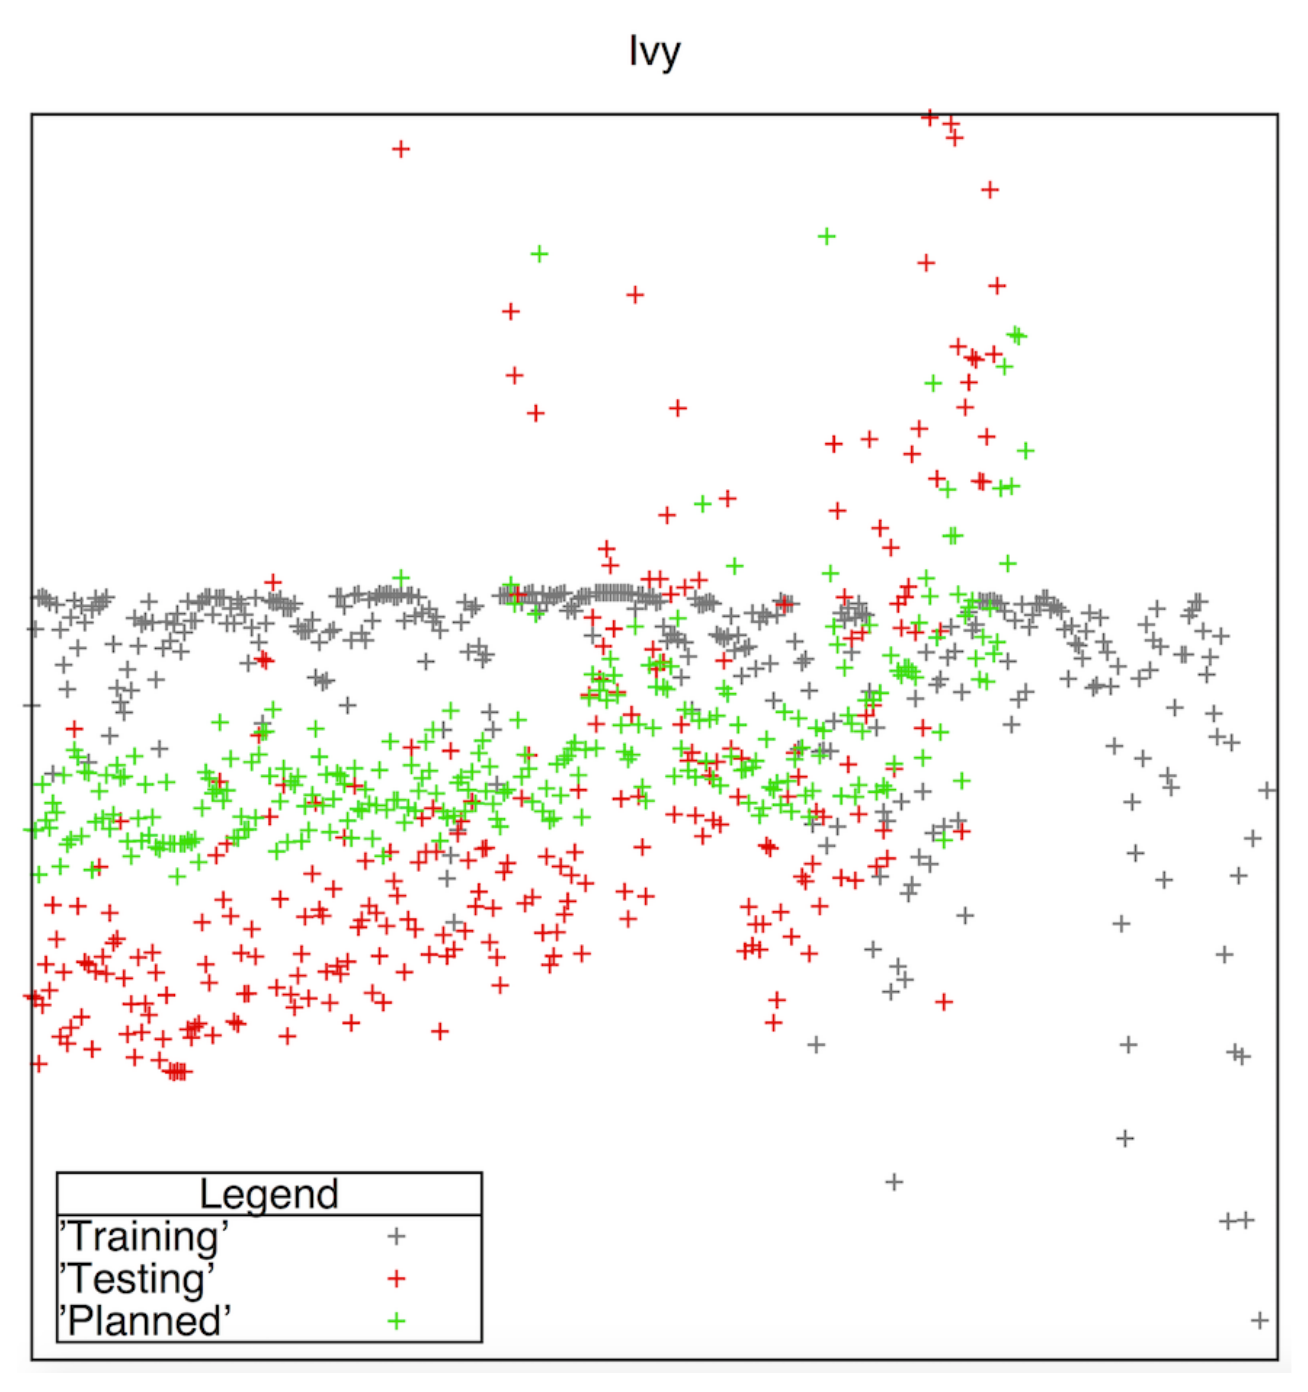
\includegraphics[width=.9\linewidth]{figs/twodee.eps} 
 % 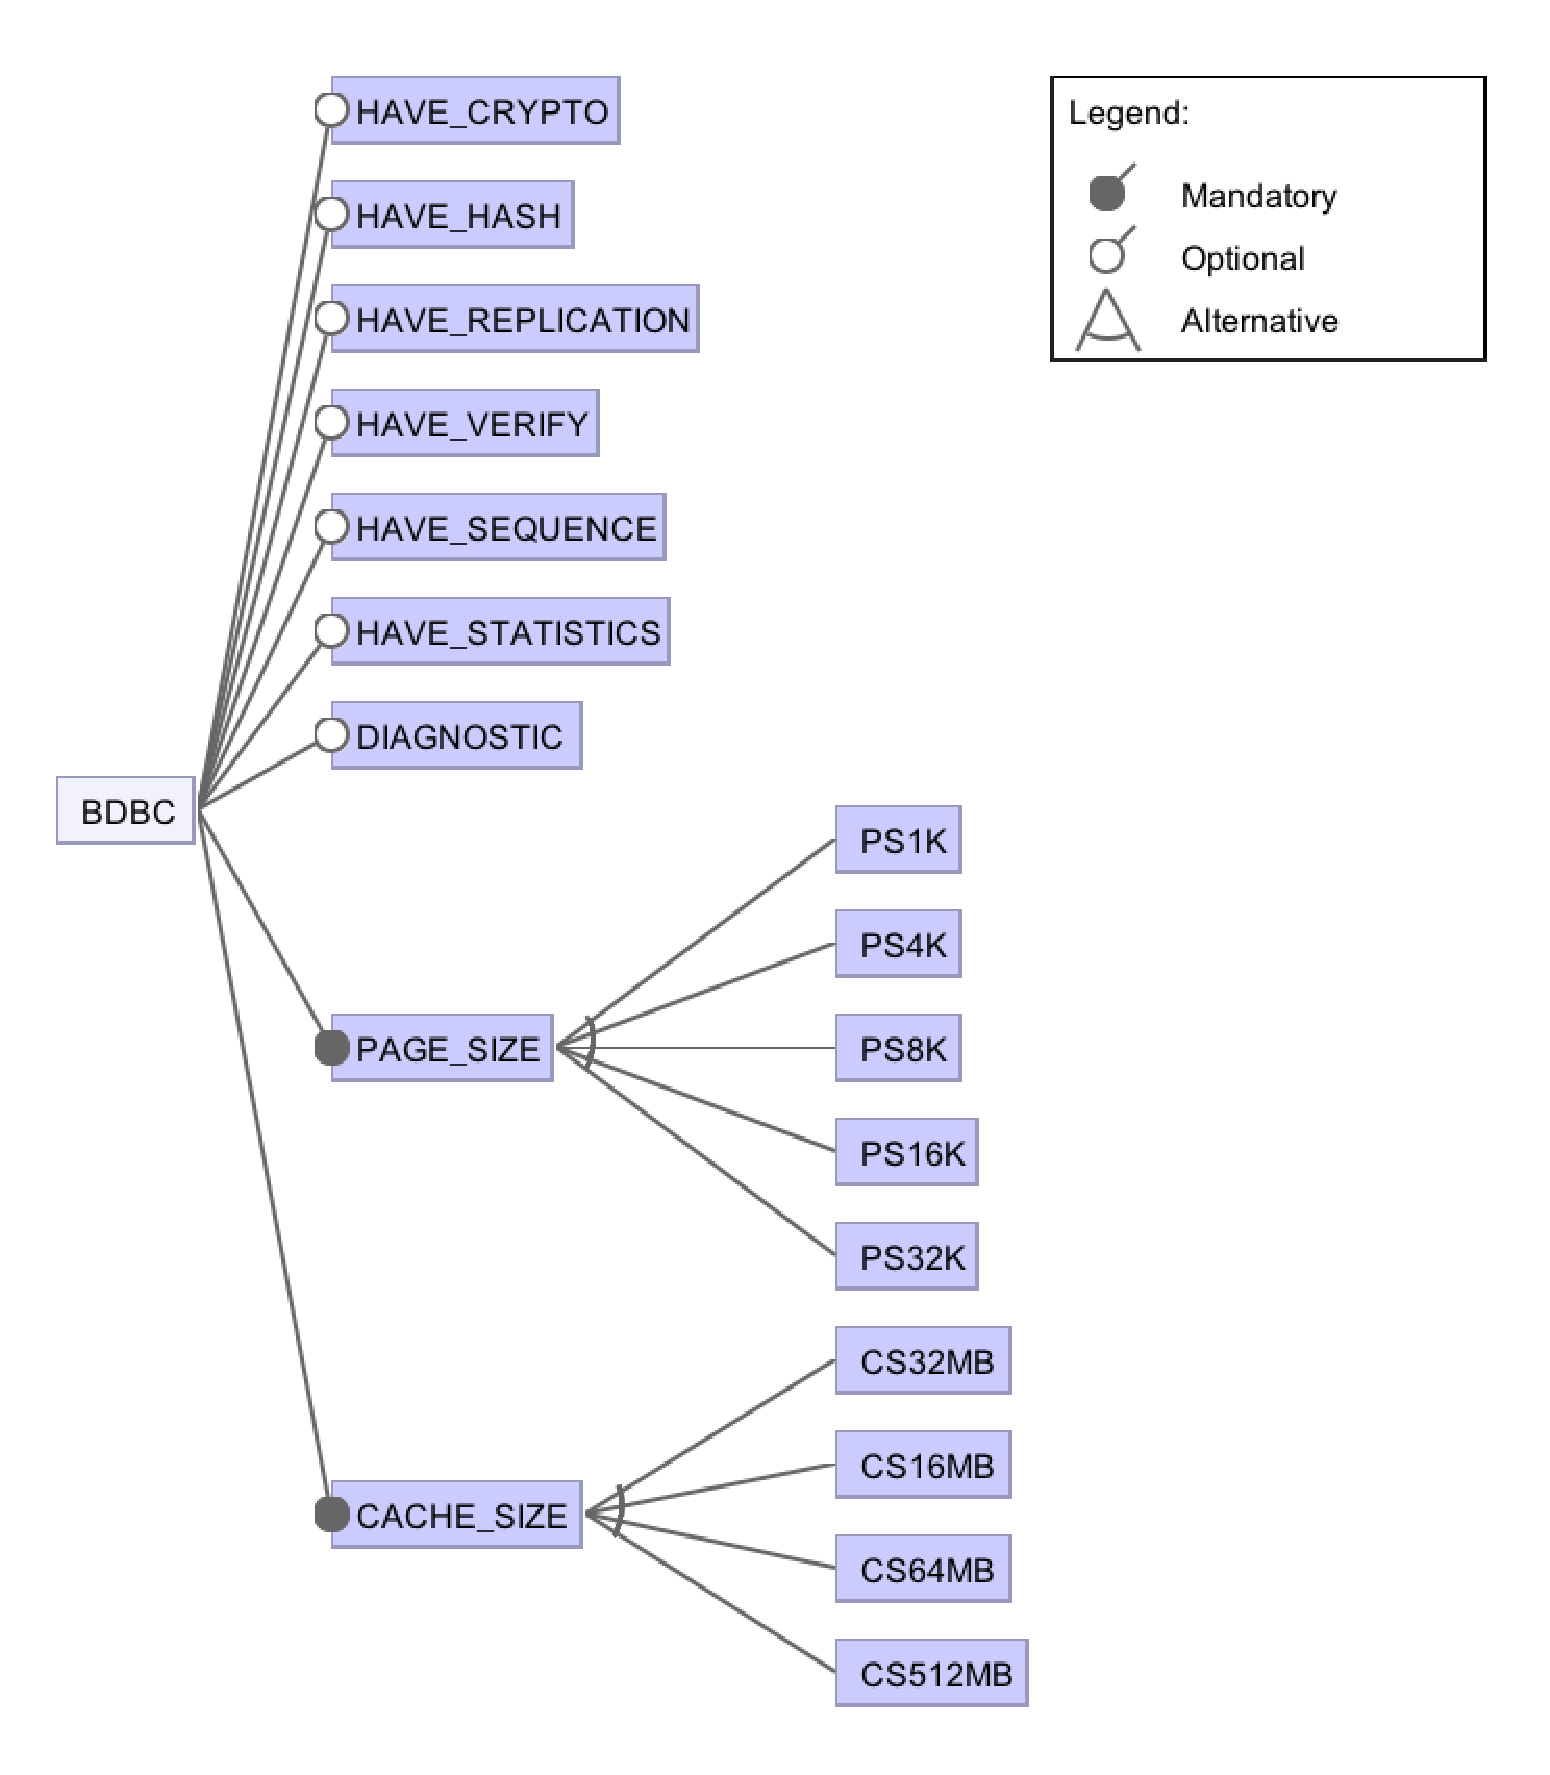
\includegraphics[width=1\linewidth]{figs/BDBC.eps}
\caption{Gray, red, green show (1) training examples, (2) test examples and 
  (3) tests that have been altered by planners.
  This figure uses axes generated from the first two components of a PCA analysis of all points. 
}\label{fig:howxy}
\end{figure}
We should mistrust the predictions made by a  model   if it is being applied to examples  that are
too far away from the
training cloud.
To test for ``too far'', we can run a data mining experiment that tests how well
a model learned from the training data applies to the test data. Such experiments return some performance value.

Note that predictions  about changes that  fall within the space of the training+test data, will be at least
as reliable as the performance value found in the above data mining experiment.
Given this, one thing  can be asserted about predictions on changed examples:
\bi
\item Predictions for changes that move examples towards/away from the training data can be trusted more/less (respectively).
\ei  
Accordingly, we should use  {\em trust-increasing} planners that generate changed examples {\em closer} to the
training examples.  To see how this works, 
 \fig{howxy} is from the {\em ivy} data
set, which is one of the Jureczko data sets explored in this paper. It shows: (1)~the training examples in gray, (2)~the test examples in red, and (3)~the
changed  examples displaced after applying a plan (in green).
 Note that the  the   changed examples
cases  (shown in green)  fall closer to the training cases (shown in gray) than
the test cases (shown in red). 

In that green region of changed examples, our belief in the value of predictions
will be as much (or more) as our belief in the value of the predictions in the red region (that
contains the original test data).
This pattern of \fig{howxy} (where the changes examples are found closer to  the training cases than the test cases) has been observed in all the other data sets studied in this
paper. Hence,  we can assert that
predictors learned from these training examples have some authority in the regions
contain the changes examples.


That said, the above comes with some important caveats:
\bi
\item 
We   strongly recommend that predictors are assessed prior to planning. That
issue is explored further in the \tion{tesd}.
\item
Planners should be designed to be {\em trust increasing}. We list four such planning methods in \tion{planners}.
\item
Where possible, planners should be assessed via some external
oracle that can accurately assess new examples. For an example of that kind of analysis,
see  \tion{coc}.
\ei

%XXX end


  
 \begin{figure}[!t]
 \small
 \begin{center}
 \begin{tabular}{r|rr}
 data set & cases & \% defective\\\hline
  ant &947& 22\\
  camel& 1819& 19\\
 jedit& 1257& 2\\
 ivy &352& 11\\
 log4j& 244 &92\\
 lucebe &442 &59\\
 poi& 936 &64\\
 synapse &379 &34\\
 velocity& 410& 34\\
 xalan& 2411& 99\\
 xerces &1055& 74
 \end{tabular}
 \end{center}
 \caption{ Jureczko data: columns in the format of \fig{ck}.}\label{fig:jd}
 \end{figure}
 
 \begin{figure}[!t]
\scriptsize
\begin{tabular}{llllll}
  \hline
  \rowcolor{lightgray}
Project & Domain & Lang. & LOC & Features & Config\\\hline
BDBC: Berkeley DB   & Database & C & 219,811 & 18 & 2560\\
BDBJ: Berkeley DB   & Database & Java & 42,596 & 32  & 400\\
Apache & Web Server & C & 230,277 & 9 & 192\\
SQLite & Database & C & 312,625 & 39 & 3,932,160\\
LLVM & Compiler & C++ & 47,549 & 11 & 1024\\
x264 & Video Enc. & C& 45,743 & 16 & 1152\\\hline
\end{tabular}
 
\caption{Siegmund data.}\label{fig:cpm}
\end{figure}

\begin{figure}[!t]
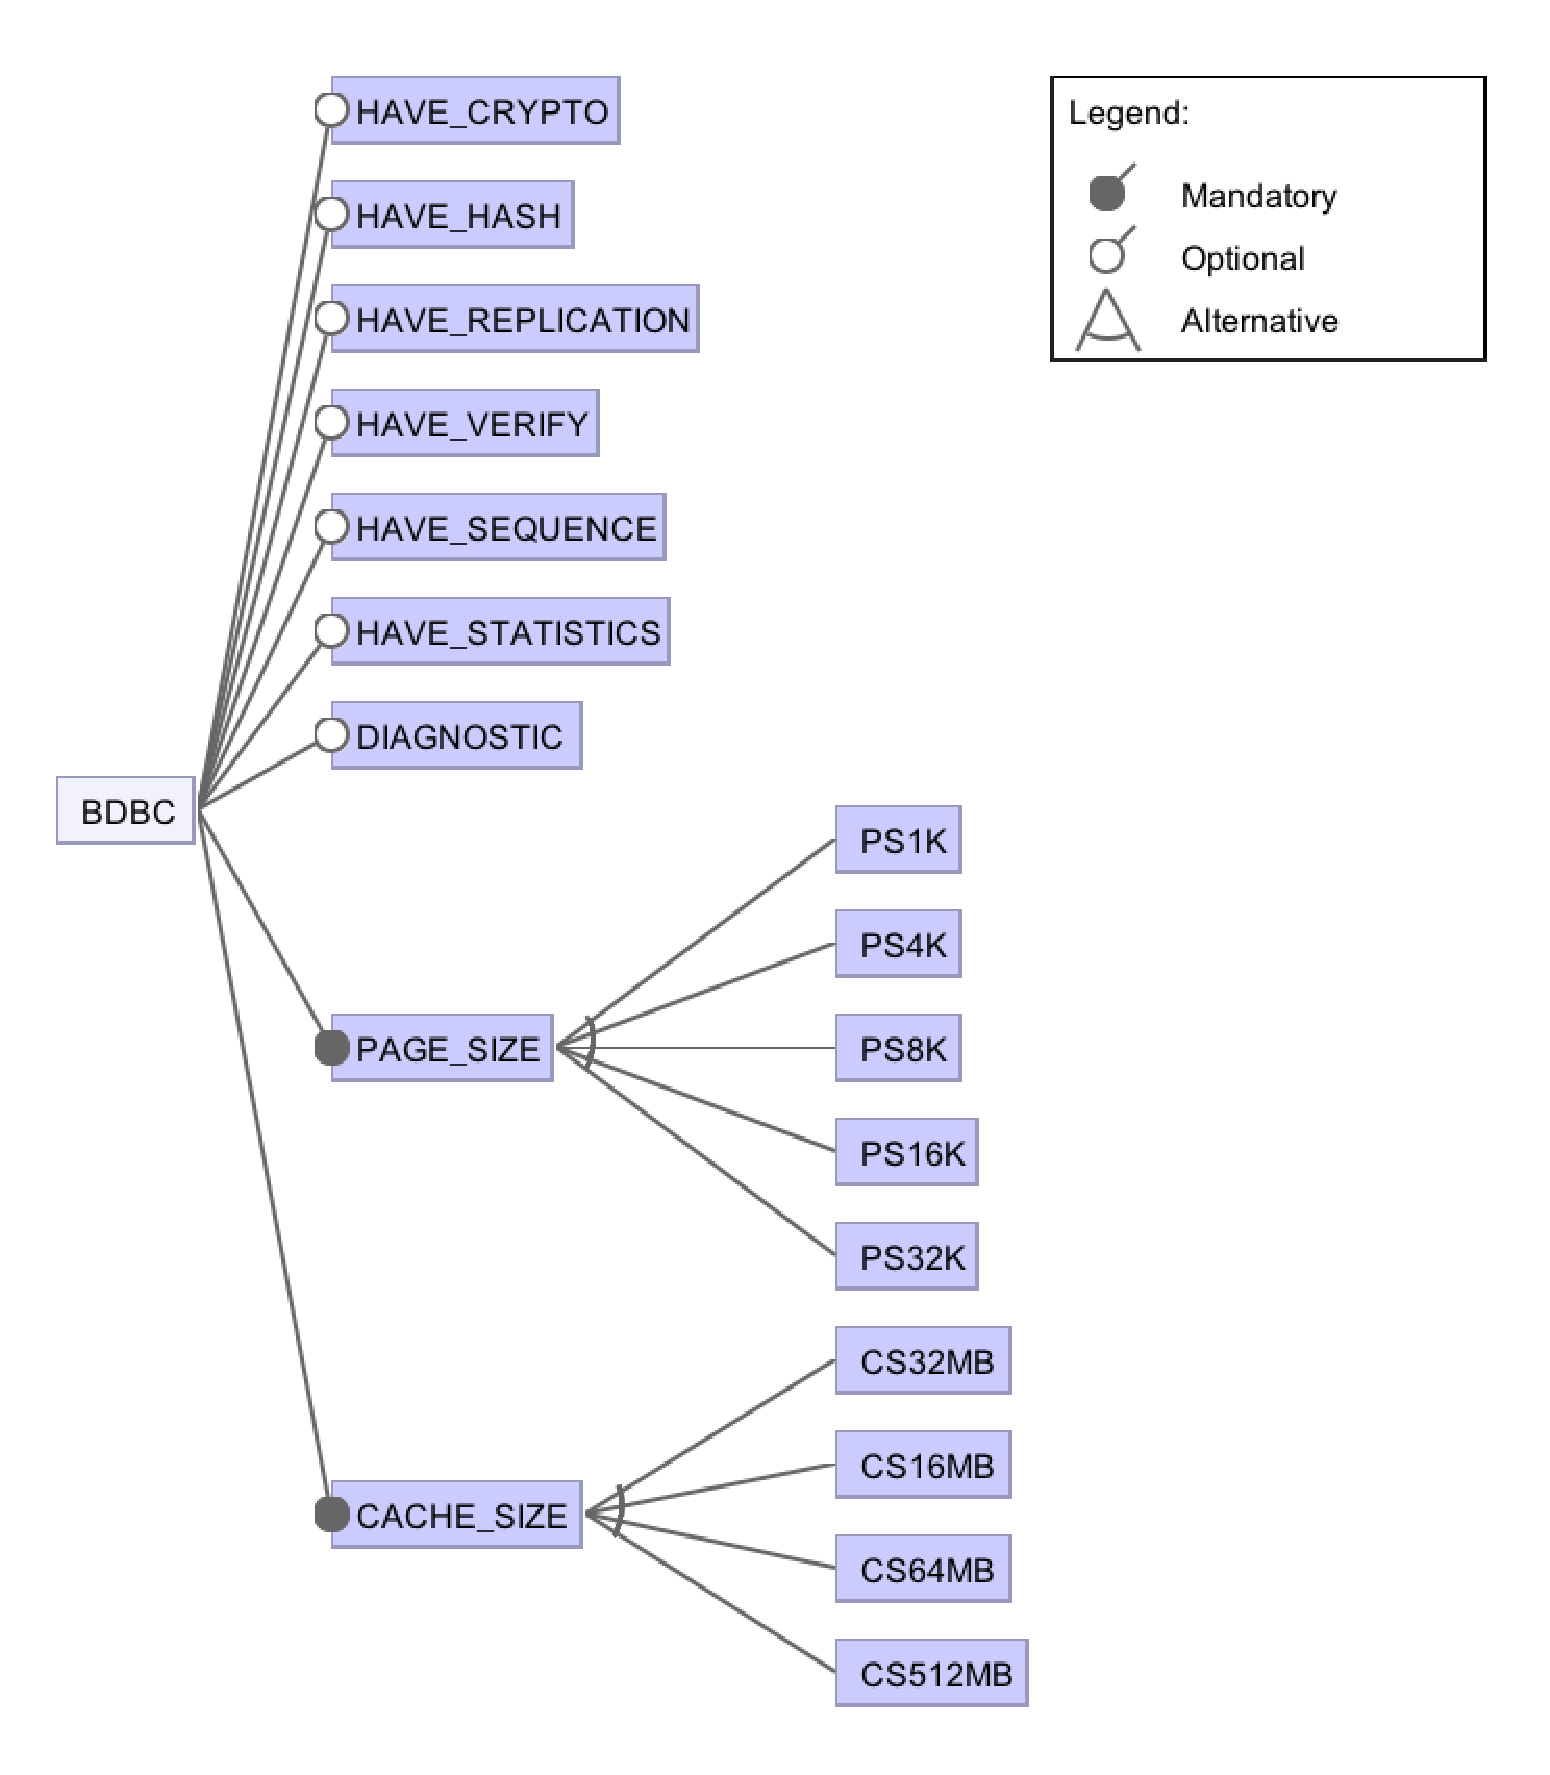
\includegraphics[width=0.9\linewidth]{figs/BDBC.eps}
\caption{ Berkeley database feature model   (``C'' version). }\label{fig:bdbc}
\end{figure}


  \section{Test Data}\label{sect:tesd}
To assess our planning methods, we use data from Jureczko et al.'s object-oriented JAVA systems~\cite{jureczko10}  and
  software system   configuration data from by  Siegmund et al.~\cite{sven12}.
  See github.com/ai-se/XTREE\#data for full access to this data.
  
  
   The Jurecko data records number of known defects for each class, where the classes are described in terms of
  nearly two dozen metrics such as number of children, lines of code, etc. For details on the Jurecko data, see  \fig{ck} and \fig{jd}. 
 For the most part, the methods of this paper treat
  the Jurecko as a discrete class data set, where {\em defects} are true if the raw defect count is greater than zero.
  The one exception will be the `best-in-cluster'' method that reflects on the numeric value of the raw defect count (see \tion{BIC}).

  The Siegmund data, described in \fig{cpm},  records  the runtimes of compiled systems. To make that data, Siegmund et al. perturbed
  the configuration parameters in the Makefiles of six systems: Apache, SQLite, LLVM, x264 and two versions of the
  Berkeley database (one written in ``C'' and one in Java). 
   \fig{bdbc} shows an example of a feature model defining valid combinations of settings to on the
   the Siegmund et al. datasets. These feature models were used by Siegmund et al. to ensure all their perturbations are value
   (we will use the same models to cull invalid plans).
  Given those valid perturbations, the systems were then compiled and 
  Siegmund et al. recorded how long each perturbation took to run a test suite. 
  
  
\begin{figure*}[!t]
	\small
	\begin{center}
		\begin{minipage}{.46\linewidth}
			\begin{tabular}{r@{~}|l@{~}|r@{~}|l@{~}|r@{~}|r@{~}|} \cline{2-6}
				& \multicolumn{5}{c|}{ }\\ 
				
				& \multicolumn{5}{c|}{ Data set  properties}\\ 
				& \multicolumn{5}{c|}{  }\\ 
				& \multicolumn{2}{c|}{training}   & \multicolumn{3}{c|}{testing}      \\ \cline{2-6}
				data set      & versions           & cases & versions     & cases    & \% defective             \\ \hline
				jedit    & 3.2, 4.0, 4.1, 4.2 & 1257      & 4.3          & 492          & 2 \\
				ivy      & 1.1, 1.4           & 352       & 2.0          & 352          & 11 \\
				camel    & 1.0, 1.2, 1.4      & 1819      & 1.6          & 965          & 19 \\
				ant      & 1.3, 1.4, 1.5, 1.6 & 947       & 1.7          & 745          & 22 \\
				synapse  & 1.0, 1.1           & 379       & 1.2          & 256          & 34 \\
				velocity & 1.4, 1.5           & 410       & 1.6          & 229          & 34 \\
				lucene   & 2.0, 2.2           & 442       & 2.4          & 340          & 59 \\
				poi      & 1.5, 2, 2.5        & 936       & 3.0          & 442          & 64 \\
			 xerces   & 1.0, 1.2, 1.3      & 1055      & 1.4          & 588          & 74  \\ 
			 log4j    & 1.0, 1.1           & 244       & 1.2          & 205          & 92   \\
			 xalan    & 2.4, 2.5, 2.6      & 2411      & 2.7          & 909          & 99  \\\hline 
				
				
			\end{tabular}\end{minipage}\begin{minipage}{.4\linewidth}
			\begin{tabular}{|rrr|rrr|rr|l} \cline{1-8}
				\multicolumn{8}{|c|}{  }\\
				\multicolumn{8}{|c|}{  Results from learning}\\
				\multicolumn{8}{|c|}{   }\\
				\multicolumn{3}{|c|}{untuned} & \multicolumn{3}{c|}{tuned} & \multicolumn{2}{c|}{change}\\
				\cline{1-8}
				
				pd & pf & good? & pd & pf & good? & pd & pf\\\cline{1-8}
				\rowcolor{celadon}55 & 29 &   & 64 & 29 & y & 9 & 0&$\star$\\
				\rowcolor{celadon}	65 & 35 & y & 65 & 28 & y & 0 & -7&$\star$\\
				49 & 31 &   & 56 & 37 &   & 5 & 6\\
				\rowcolor{celadon}	49 & 13 & y & 63 & 16 & y & 14 & 3&$\star$\\
				45 & 19 &   & 47 & 15 &   & 2 & -4\\
				78 & 60 &   & 76 & 60 &   & -2 & 0\\
				56 & 25 &   & 60 & 25 & y & 4 & 0\\
				\rowcolor{celadon}	56 & 31 &   & 60 & 10 & y & 4 & -21&$\star$\\
			\rowcolor{lavenderpink}	30 & 31 &   & 40 & 29 &   & 10 & -2&$\times$\\
				\rowcolor{lavenderpink}32 & 6 &   & 30 & 6 &   & -2 & 0&$\times$\\
				\rowcolor{lavenderpink}38 & 9 &   & 47 & 9 &   & 9 & 0&$\times$\\
				\hline 
			\end{tabular}
			
		\end{minipage}
	\end{center}    
	
	\caption{Training and test {\em data set properties} for  Jureczko data ,
		sorted by \% defective examples.
		On the right-hand-side, we show the {\em results from learning}.
		Data is usable if it has a recall of 60\% or more and false alarm of 30\% or less (and note that, after tuning, there are more usable data sets than before). Results  	\colorbox{celadon}{ marked with ``$\star$''} show large improvements in performance, after tuning
		(lower {\em pf} or higher {\em pd}).
		Data in  the  \colorbox{lavenderpink}{three bottom rows}, marked with ``$\times$'', are  performing
		poorly-- that data so few non-defective examples  that it  is hard for
		our learners to distinguish between classes.
	}\label{fig:j}
\end{figure*}


  Our evaluation strategy (discussed below) divides this data into a training a test set.
  From the train set we apply a data miner (to learn a quality predictor) and
  various planning methods (to learn different plans). Next, we try applying
  each of those plans to the  test set and ask the quality predictor to assess the changed examples.
  Finally, we say that the  ``best'' planner is the one that most reduces the predicted values
  in the changed examples.
  
  As mentioned in the last section,  this approach depends on having effective predictors for assessing the results.
  For the Siegmind data, this criteria was   relatively easy to achieve.
  The data in those data sets have a continuous class (runtime of the compiled system)
  so the performance of a quality predictor can  be measured in terms of  difference between the predicted runtime $p$ of test case items and their actual runtimes $a$ using  $s= 1 - \frac{abs(a - p)}{a}$ (and {\em higher} values are {\em better}).
This paper  explores six Siegmund configuration data sets:  Berkeley DB (Java and C versions), Apache, SQLite, LLVM, and
  x264. 
  As a preliminary study, we split that data   into equal sized train:test groups
  and trained a Random Forest
  Regressor (from the SciKit learn kit~\cite{Pedregosa2012})   on one half, then applied to the other. This  achieved nearly perfect scores of $s=\{99.9, 99.8, 99.4, 99.1, 96.1\}\%$.
That is, we can be very confident that the predictors from the Siegmund data can assess
our plans. (Aside: if the reader doubts that such high scores are achievable, we note that these scores are consistent with those achieved by predictors built by Siegmund et al.~\cite{sven12}.)



 It proved to be  more complicated to commission the Jureczko data sets for this study.
 For that data, we found that the
 quality predictors built from this data are far from perfect;
However, for some data sets, the  predictors could
be salvaged using the techniques discussed in this section.

 \fig{j} shows our preliminary studies with the Jureczko   data.
Given access to $V$ released
versions, we test on version $V$ and train on the available data from $V-1$ earlier releases (as
shown in \fig{j}, this means that we are training on hundreds to thousands
of classes and testing on smaller test suites).
Note the   \colorbox{lavenderpink}{three bottom rows}   marked with $\times$: these contain predominately
defective classes (two-thirds, or more).  In such data sets, it is hard to distinguish
good from bad (since there are so many bad examples). 


The  Jureczko data uses non-numeric discrete classes (``defective'' or ``not'').
For such data, quality predictor   is be measured using
(1) the  probability of detection (a.k.a. ``pd'' or recall):  the percent of faulty classes in
the test data detected
by the {\em predictor}; and (2) the 
probability of false alarm (a.k.a. ``pf''): the percent of non-fault
classes that are {\em predicted} to be defective.

As a preliminary study, we split the Jureczko  data   into equal sized train:test groups.
Random Forests (again, from the SciKit learn kit~\cite{Pedregosa2012}) were
built from the training data, then applied to the test data.
The ``untuned'' columns of \fig{j} shows those results.
If we define ``good'' to mean $\mathit{pd}>60 \wedge \mathit{pf} < 40$\%,
then only two of our data sets ({\em ivy,ant}) are ``good'' enough for this study.
Note that, as might have been expected, none of the \colorbox{lavenderpink}{three bottom rows} of \fig{j} were ``good''.

Fortunately,
the ``tuned'' columns of \fig{j} show that we can salvage some of the data sets. Pelayo and Dick~\cite{pelayo07} report that defect prediction is improved by SMOTE~\cite{Chawla2002}; i.e. an over-sampling of minority-class examples. Also, Fu et al.~\cite{fu:ase15} report that parameter tuning with differential evolution~\cite{storn97} can quickly explore the tuning options of Random Forest to find better settings for the (e.g.) size of the forest, the termination criteria
for tree generation, etc. The rows \colorbox{celadon}{marked with a $\star$} in \fig{j} show data sets whose performance was improved remarkably by these techniques. For example, in {\em poi}, the recall increased by 4\% while the false alarm rate dropped by 21\%. However,  as might have been expected, we could not salvage the data sets in the  three bottom rows.

In summary, while we cannot trust predictors from some of our defect data sets,
we can plan ways to reduce defects in {\em jedit, ivy, ant, lucene} and {\em poi}.
Accordingly, when this study explores the Jureczko data, we will use these five data sets.

(Aside: One important detail to be stressed here is that, when we applied    SMOTE-ing and
parameter tunings, those techniques were applied to the training data and {\em not}
the test data; i.e. we took care that no clues from the test set were ever used in this tuning process.)



 
\section{Four Planning Methods}\label{sect:planners}
 
This section described XTREE (which we call Method4) and  three  
alternate methods for learning plans.
  XTREE  uses the decision tree learner of \fig{where}.D.  It is new to this paper.
  The other methods use the   top-down
	bi-clustering method described in \fig{where}.C  which recursively divides the
	data in two  using a dimension that captures the greatest variability in the data. 
	We proposed Method 1 and 2   in 2012~\cite{me12c} while Methods 3 comes from research conducted earlier this year~\cite{krishna15}.
 
 
  Note that all   methods have the  properties proposed in \tion{prelim}.
  That is, they are {\em local learners}; i.e. different test examples
  will be given plans that are specialized  to their particulars. Also,
  they  are {\em trust-increasing}; 
  i.e. they change  examples such that they move {\em closer} to the training data.
 

 \subsection{  Methods}

Our  description of the methods adopts the following convention. All variables
  set via  our engineering judgement  with Greek letters; e.g. $\alpha,\beta,\gamma$.
  In this paper, we show our current settings to these variables produces useful
  results. Elsewhere\cite{krall14,fu:ase15}, we are exploring tuning methods to 
  find better settings but  we have nothing definitive yet to report
  on auto-tuning planners.

\subsubsection{Method1= CD=   Centroid Deltas}


 {\em Summary1:} Method1  computes a plan from the difference between where you are  (which we will call $C_i$) and
where you want to be  (which we will call $C_j$).

{\em Assumption1: } Method1 assumes that large data sets can be adequately represented by a few dozen (or so) 
centroids.
 
 {\em Details1:} Method1 clusters project data by reflecting   on the independent variables, then
  reports the delta between the cluster centroids. 
  After clustering   training data using the WHERE algorithm of  \fig{where}.C, Method1
replaces all clusters with a  centroid $C_i$ computed from the mean/mode value of each
continuous/discrete feature. After that, it
finds the closest centroid $C_j$ that has a better
performance score. For defect data, ``better'' means fewer defective examples while for the config data,
``better'' means lower median runtimes for the examples in that cluster.
Method1 then caches the  delta between the independent features between $C_i$ and $C_j$. For continuous
features, this delta is $C_j - C_i$. For discrete values, this delta is the value of that feature
in $C_j$. 
Finally, for every test case, Method1 use the distance measure $d$ shown in \fig{where}.B to find
the nearest centroid $C_i$.  It then proposes a plan for improving that test case
that is the conjunction of all the deltas between $C_i$ and $C_j$.


\subsubsection{Method2=CD+FS=Method1+Feature Selection }
 
{\em Summary2:} Method2 works line Method1 but now the   plans  only
mention the $\beta=33\%$ most informative features. Hence, Method2's plans are simpler.

{\em Assumption2: } Method2 assumes that, when reasoning about centroids, we can
just use   features
that   best distinguish    centroids; i.e. whose values appear in just a few centroids.
 

{\em Details2:} A common result is that the signal in a table of data is mostly contained in a handful of features~\cite{hall03,kohavi97}.
Papakroni~\cite{papa13} has tested for this effect in the Jureczko data sets.
Papakroni found no loss of   efficacy in defect prediction after
sorting all features by their information content,
then making predictions using (a)~all  features or (b)~just using   33\% most informative features.

Based on the above, it might be possible to simplify the plans found by Method1  by pruning back the features in those
 plans. Following on from Papakroni, our Method2 returns plans
containing just the top $\beta=33\%$ most informative features. Here, ``informative'' means
that the values of a feature are good for selecting a small set of clusters (ideally,
just one).
This can be estimated using the Fayyad-Iranni INFOGAIN algorithm~\cite{FayIra93Multi}
of \fig{where}.E.
 
 
 
	\begin{figure} 
	\begin{shaded}
  ~\hrule~
  
 {\bf Figure 7.A: Measuring Variability} 
	
	For  continuous and discrete values,
the {\em variability} can be measured using standard deviation $\sigma$ or entropy $e$.
Note that \mbox{$\sigma = \sqrt{\sum^n_{i=1} \left( \frac{x_i - \bar{x})^2}{n-1}\right)}$}
where $\bar{x}$ is the mean of  numeric features $x_1,x_2,..x_n$.
Also \mbox{$e = - \sum^n_{i=1} p_i \mathit{log}_2(p_i)$} 
for  $n$ discrete values  at frequency
$f_1,f_2,.. f_n$ for \mbox{$N = \sum^n_{i=1} f_i$} and $p_i = f_i/N$.

  ~\hrule~
	
	{\bf Figure 7.B: Measuring distance}
	
	We use
		 Aha et al.'s standard Euclidean distance measure~\cite{aha91}.  For $F$ independent features, the measure returns   $d(X,Y)=\sqrt{\sum_i^F  w_i\Delta(X_i,Y_i)^2}$. Here, $w_i$ is a weight term for each feature
		 (usually set to 1).
			Within $\Delta$, if   $X_i,Y_i$ are both missing  values, then  return 1.
			Otherwise, replace any  missing items with values that maximizes the following.
			For numerics $\Delta$ normalizes $X_i,Y_i$ (to the range 0,1 for min,max) then
			returns 
			$X_i - Y_i$. For discrete variables, $\Delta$ returns 0,1 if $X_i,Y_i$ are the
			same,different (respectively).  

 ~\hrule~
 
	{\bf Figure 7.C: Top-down Clustering with WHERE}
	
				WHERE  divides data into  groups of size $\alpha=\sqrt{N}$ using 
		Using this measure, WHERE runs as follows:
		\begin{enumerate}[leftmargin=3mm]
			\item Find   two   distance cases,  $X,Y$
			by picking any case $W$ at random, then setting $X$ to its most
			distant case, then setting $Y$ to the case most distant from
			$X$
			(which requires only $O(2N)$ comparisons).
			\item Project each case $Z$
			to position $x$ on a    lines running from $X$ to $Y$: if $a,b$  are distances  $Z$ to $X,Y$  then  $x = (a^2+c^2 - b^2)/(2ac)$.
			\item Split the data at the median $x$ value of all cases.
			\item For   splits larger than  $\alpha=\sqrt{N}$, recurse   from step1.
		\end{enumerate}
 In terms of related work,
	  the above is similar in approach to Boley's PDDP algorithm~\cite{boley98}, but PDDP requires an $O(N^2)$ calculation
	  at each recursive level to find the PCA principle component. Our method, on the other hand,
	  performs the same task with only $O(2N)$ distance calculations 	using the 
	  FASTMAP heuristic~\cite{Faloutsos1995} shown in step1. Platt~\cite{platt05} notes that FASTMAP is a  Nystr\"om approximation to the first component of PCA.  
	  
	   ~\hrule~
	   
	{\bf Figure 7.D: Top-down division with Decision Trees}
	
	Find a split in the values of  independent features that most reduces the variability
  of the dependent feature (measured using \fig{where}.A). w
	
	 ~\hrule~
	 
	 	{\bf Figure 7.E: Finding the most informative rows}
	

Discretize all numeric features using the Fayyad-Iranni discretizer~\cite{FayIra93Multi}
(divide numeric columns into bins $B_i$, each of which  select for the fewest cluster ids).
Let feature $F$ have bins $B_i$, each of which contains $n_i$ rows
and 
let each bin $B_i$ have entropy $e_i$ computed from the frequency of clusters seen in that bin (computed from \fig{where}.A).
Cull the the features as per Papakroni~\cite{papa13}; i.e. just use the $\beta=33\%$ most informative features
where  the   value of  feature $F$ is $\sum_i e_i\frac{n_i}{N}$ ($N$ is the number of rows).

~\hrule~ 

	  \end{shaded}
		\caption{Some algorithms used in this paper.}\label{fig:where}
		\end{figure}
\subsubsection{Method3= BIC=   Method2 + Best-in-cluster}\label{sect:BIC}

{\em Summary3:} Method3 is like Method2, but it uses more knowledge about the training data.

{\em Assumption3: } Method3 assumes that there exists ``gradients'' between and
within clusters which, if used, will better guide us to finding better plans.

{\em Details3:}
Method3 summarizes clusters into {\em two} examples: (1)~the centroid $C_x$ found in Method1 and
(2)~the best-in-cluster $B_x$  example; i.e. the  example in that cluster
with the best performance score. 
For the Siegmud data, $B_x$ is the cluster member with the fastest runtime;
for the Jureczko data, $B_x$  is the cluster member with lowest raw defect count
(resolving ties at random).

Method3 connects  each centroid to a nearest neighbor
by a {\em gradient}.
Each gradient has a (bottom,top) end labelled  ($C_i,C_j$) containing the  (worst,best) centroid performance scores, respectively..  
For each test instance, Method3 
find the nearest gradient, the runs up to the top  best end $C_j$, then extracts $B_j$ (which is the
 best-in-cluster associated with  $C_j$).
The returned plan is then computed  from the delta between the test case
and $B_j$.
 
%\begin{figure}[t] 
~\hrule~
\begin{minipage}[t]{.45\linewidth}
% \scriptsize\vspace{1mm}
\begin{code}[left]
def kNN(training, testing, F=33):
  """ Identify contrast sets for testing
      data using Nearest Neighbor """
  def exemplar(rows):
    return centroid(rows)
  
  def nearest(me, clusters):
    return sorted(clusters,
                  key=lambda F: dist(exemplar(F), me))
  
  def envy(me, clusters):
    one=exemplar(nearest(me, clusters))
    better=[c for c in clusters if score(c)<score(one)]
    two=exemplar(nearest(one, better))
    return one, two
  
  def Prune(list, Frac):
    "Return top Frac % of the list"
    
  def contrastSet(t):
    clusters = WHERE(training)
    one, two = envy(t,clusters)
    return Prune(one-two, Frac=F)
  
  # ---- Begin Main Code ---------------
  return [contrastSet(t) for t in testing]
\end{code}
\end{minipage}
~\hrule~
\caption{Nearest Neighbor (Python-style psuedo-code).
For brevity's sake, this code skips certain low-level details.
For a full working implementation, see \url{http://git.io/v36sb}.}
\label{fig:knncode}
\end{figure}


\begin{figure}[!t] 
	\begin{shaded}
  ~\hrule~
	
Using the training data,  divide the data using the decision tree of algorithm of \fig{where}.D into groups of
size $\alpha=\sqrt{N}$.

For each item in the test data,
	  find the {\em current } leaf: take each test instance, run it down to a leaf in the decision tree.  
After that,	  find the {\em desired} leaf:
		\begin{itemize}[leftmargin=3mm]
		\item Starting at {\em current}, ascend the tree $lvl\in \{0,1,2...\}$ levels;
		\item Identify {\em sibling} leaves; i.e. leaf clusters that can be reached from level $lvl$ that are not {\em current }
		\item Using the {\em score} defined above, find the {\em better} siblings; i.e. those with a {\em score} less than $\gamma=0.5$ times the mean score of {\em current}.
		 \bi
		 \item 
		   If none found, then repeat for $lvl += 1$
		 \item
		    Return no plan if the new $lvl$ is above the root.
		 \ei
		\item  Return the {\em closest} better sibling where distance is measured between the mean centroids of that sibling and {\em current}
		\ei
	 Also, find the {\em delta}; i.e. the set difference between  conditions in the decision tree branch to {\em desired} and {\em current}. To find that delta:
		\begin{itemize}[leftmargin=3mm]
		\item
		For discrete attributes,  return the value from {\em desired}. 
		\item
		For  numerics, return the numeric difference. 
		\item
		For numerics  discretized into ranges, return a random number selected from the low and high boundaries of the that range.
		\ei 
		Finally, return the delta as the plan for improving the test instance.
		~\hrule~
		\end{shaded}
		\caption{XTREES}		\label{fig:xtrees_bare}
	\end{figure}


\subsubsection{Method4=XTREE=  Deltas in Decision   Branches}

{\em Summary4:} Method4 builds a decision tree,  then generates
plans from the difference between two branches:
(1)~the branch to where you are and (2)~the branch to where you want to be.

{\em Assumption4:} One potential problem with Methods 1,2 and 3 is the {\em unsupervised} nature of
the clustering algorithm (WHERE) that  
executes without knowledge of the target class.  {\em Supervised} methods, on the other hand, assume that it is useful to also reflect on the target class.

{\em Details4:} 
XTREE uses a supervised   decision tree algorithm of \fig{where}.D to divide the data.
Next, XTREE builds plans from the branches of the decision trees using the code of \fig{xtrees_bare}.
That code asks three questions, the last of which returns the plan:
\be
\item
What {\em current} branch does a test case fall in?
\item What {\em desired} branch would the test case want to move to?
\item What are the {\em deltas} between current and desired? 
\ee
 
\newpage \section{Experiments}

  
 

This section describes an experimental design (and results) for evaluating the above four methods. 
\subsection{Experimental Design}

\subsubsection{A Strategy for Evaluating Planners}
 
 Here is our experimental design:
 
 \begin{figure}[!h]
{\small 
\[
\begin{array}{r} 
\mathrm{project}\\
\mathrm{data}
\end{array} 
\left\{\begin{array}{l}\mathit{train}
        \left\{\begin{array}{l}
                \mathrm{learn\;a\;}\mathrm{predictor\;}\mathrm{(e.g.\;via \;Random\;Forest)}\\
                \mathrm{learn\;a\;}\mathrm{planner\;}\mathrm{(e.g.\;via \; XTREE)}
              \end{array}\right.
       \\
      ~\\
\mathit{test}  
    \left\{\begin{array}{l@{~}l}
           \mathit{before}& =\mathrm{Performance\; scores \hspace{2pt} in \hspace{2pt}}\mathit{test}\\
           \mathrm{\bf if\;}\mathit{before} & >  \mathit{0}\\
           \mathrm{\bf then} &
           \left\{
            \begin{array}{l}
                \mathit{test'} = \mathrm{planner}(\mathit{test})\\
                \mathit{after} =\mathrm{predictor}(\mathit{test'})\\ 
                \mathrm{{\bf return}\;} R=\frac{\mathit{after}}{\mathit{before}}
            \end{array}
          \right.
   \end{array}\right.
\end{array} \right. 
\]}
 \caption{Experimental .}\label{fig:design}
 \end{figure}

As shown in \fig{design}, we divide the
project data  into two disjoint sets {\em train} and {\em test}
(so \mbox{{\em train} $\cap ${\em test} $=\;\emptyset$}).
Next, from the train set, we build both a {\em planner} and
 a {\em  predictor}. 

Our general framework does not   commit to any particular choice of { planner} or { predictor} but, for the purposes of this paper:
\bi
\item Our {\em planner} will be one of Methods 1,2,3,4;
\item Our  {\em predictor} will be the Random Forest Classifier~\cite{Breiman2001} (for discrete classes) and Random Forest Regressor (for continuous classes) taken from  SciKit Learn~\cite{Pedregosa2012}.   We use these
data miners since extensive studies have shown these to be amongst the better alternatives for mining software data~\cite{lessmann}.
\ei
As for the {\em test} data, this is passed to the { predictor}
to measure performance statistics related to effectiveness. 

If our { predictors} fail to perform effectively on the test data,
then we cannot trust them to comment on our plans. Accordingly,
if that performance is unsatisfactory, we abort. Recall from \tion{tesd} that this step indicated
we should not use some of the  Jureczko data.

Else, we (1)~apply the { planner} to alter the {\em test} data;
then (2)~apply the { predictor} to the altered data $test'$;
then (3)~return data on the {\em before, after} predictions expressed as the ratio $R=\frac{\mathit{after}}{\mathit{before}}$.
This is a unit-less ratio with the following properties:
\bi
\item If $R= 1$, this means  ``no change from baseline''; 
\item If $R < 1$, this indicates ``some reduction to the baseline'';
\item If $R > 1$, this indicates ``optimization failure''.
\ei
 \subsubsection{Statistical Methods}
 Our methods use some stochastic algorithms; e.g. WHERE's selection of ``what example to explore first'' (see \fig{where}.C) and
  XTREE' occasional use of a random guess when deciding what part of a discretized range to include in the plan
  (see \fig{xtrees_bare}). Hence, we report the $R$ values seen in 40 repeated runs
  (with different random number seeds).
The the value 40 was chosen to be  larger than the 30 samples  required
to satisfy the central limit theorem.

  To rank our methods using the results from these 40
  repeats, we use the Scott-Knott test recommended by Mittas and  Angelis~\cite{mittas13}. 
In that test, using the median values of each method,  
sort a list of  $l=40$ values of $R$ values found in  $ls=4$ different methods. 
Then,
splits $l$ into sub-lists $m,n$ in order to maximize the expected value of
 differences  in the observed performances
before and after divisions. E.g. for lists $l,m,n$ of size $ls,ms,ns$ where $l=m\cup n$:
 \[E(\Delta)=\frac{ms}{ls}abs(m.\mu - l.\mu)^2 + \frac{ns}{ls}abs(n.\mu - l.\mu)^2\]
Scott-Knott  applies an statistical  hypothesis test $H$ to check
if $m,n$ are significantly different  (in our case, the conjunction of A12 and bootstrapping). 
If so, Scott-Knott  recurses on the splits.
In other words, the Scott-Knott procedure being used here divides the data if \textit{both} bootstrap sampling and effect size test agree that a division is statistically significant (with a confidence of 99\%) and not a small effect ($A12 \ge 0.6$).

For a justification of the use of non-parametric bootstrapping, see Efron \& Tibshirani~\cite[p220-223]{efron93}. For a justification of the use of effect size tests see Shepperd\&MacDonell~\cite{shepperd12a}; Kampenes~\cite{kampenes07}; and Kocaguenli et al.~\cite{Kocaguneli2013:ep}. These researchers warn that even if an hypothesis test declares two populations to be ``significantly'' different, then that result is misleading if the ``effect size'' is very small. Hence, to assess the performance differences we first must rule out small effects using A12, a test   recently endorsed by Arcuri and Briand at ICSE'11~\cite{arcuri11}.



\subsubsection{Report Format}

   
Our results are presented by the line diagrams like those shown on the right-hand-side of the following example table.
The black dot shows the median $R$ value and the horizontal likes stretch over the inter-quartile
range (hereafter, IQR) that is the space from the 25th percentile value to
the 75th percentile value.

\begin{center}

{\small  \begin{tabular}{{l@{~~~~}l@{~~~~}r@{~~~~}r@{~~}c@{}r}} 
\arrayrulecolor{lightgray}
\textbf{Rank} & \textbf{Treatment} & \textbf{Median} & \textbf{IQR} & \\\hline
1 &         XTREE &    0.49  &  0.13 & \quart{7}{25}{17}{115} \\\hline  
2 &      CD &    0.59  &  0.18 & \quart{15}{34}{36}{115} \\
2 &          BIC &    0.60  &  0.12 & \quart{24}{24}{38}{115} \\\hline  
3 &      CD+FS &    0.62  &  0.06 & \quart{36}{12}{42}{115}  \\\hline \end{tabular}}
\end{center}

In this example table, the rows are  sorted on the median values of each method. Note that all the methods
have   $R<1$ values; i.e. all these methods reduced the expected value of the performance score in that experiment
while XTREE achieved the greatest reduction (down to 49\% of the original value).


The above eample table has a  left-hand-side  {\bf Rank} column, computed using the
Scott-Knott test described above. This column reports if
the values for each method are statistically different and are more than trivially different. 
In this example table, CD and BIC are ranked together while XTREE and CD+FS are ranked best and worst, respectively.
  
 

 
\subsubsection{Other Details}
 
\fig{jur} and \fig{conf1} show the effectiveness of our methods seen in 40 repeats with each data set.
In these experiments,   the dependent variables of Jureczko and Siegmund data sets are discrete and continuous in nature, respectively. Hence, while choosing the predictor, we used Random Forest (1) as a classifier for Jureczko data and (2) as a regressor for Siegmund data.
\bi
\item For Siegmund data, we randomized the order of the data, training on one half while identifying treatment plans on the remaining test data. 
\item For the Jureczko data, we used the training and testing sets of \fig{j}. For these datasets,
 all the SMOTE-ing and Random Forest tunings (discussed in \tion{tesd})
occurred in the {\em train} phase of \fig{design}.
\ei
 \subsection{Experimental Results}

Recall from our introduction that we are assessing planners on three criteria:
{\em effectiveness}, which is how much they reduce the expected value of the changed examples;
{\em succinctness}, which is how many things we need to change to achieve a plan;
and {\em surprise}, which is how different are the plans from standard truisms.

\begin{figure}[!b]
{\small \textbf{Ant}\\[0.1cm]}
  {\small  \begin{tabular}{{l@{~~~~}l@{~~~~}r@{~~~~}r@{~~}c@{}r}}

\arrayrulecolor{lightgray}
\textbf{Rank} & \textbf{Treatment} & \textbf{Median} & \textbf{IQR} & \\\hline
  1 &        XTREE &    60  &  8 & \quart{44}{7}{47}{79} \\
\hline  2 &           CD &    52  &  15 & \quart{33}{12}{41}{79} \\
\hline  3 &        CD+FS &    45  &  1 & \quart{35}{1}{35}{79} \\
  3 &          BIC &    45  &  3 & \quart{34}{2}{35}{79} \\
\hline \end{tabular}}\\[-0.1cm]

{\small \textbf{Lucene}\\[0.1cm]}
  {\small  \begin{tabular}{{l@{~~~~}l@{~~~~}r@{~~~~}r@{~~}c@{}r}}
\arrayrulecolor{lightgray}
\textbf{Rank} & \textbf{Treatment} & \textbf{Median} & \textbf{IQR} & \\\hline
  1 &        XTREE &    57  &  8 & \quart{42}{6}{45}{79} \\
\hline  2 &           CD &    49  &  5 & \quart{36}{4}{39}{79} \\
  2 &        CD+FS &    49  &  5 & \quart{37}{4}{39}{79} \\
\hline  3 &          BIC &    46  &  2 & \quart{35}{2}{36}{79} \\
\hline \end{tabular}}\\[-0.1cm]

{\small \textbf{Poi}\\[0.1cm]}
  {\small  \begin{tabular}{{l@{~~~~}l@{~~~~}r@{~~~~}r@{~~}c@{}r}}
\arrayrulecolor{lightgray}
\textbf{Rank} & \textbf{Treatment} & \textbf{Median} & \textbf{IQR} & \\\hline
  1 &        XTREE &    56  &  1 & \quart{40}{8}{44}{79} \\
\hline  2 &           CD &    44  & 16 & \quart{29}{13}{35}{79} \\
  2 &          BIC &    43  &  9 & \quart{30}{7}{34}{79} \\
  2 &        CD+FS &    40  &  5 & \quart{30}{4}{31}{79} \\
\hline \end{tabular}}\\[-0.1cm]

{\small \textbf{Ivy}\\[0.1cm]}
  {\small  \begin{tabular}{{l@{~~~~}l@{~~~~}r@{~~~~}r@{~~}c@{}r}}
\arrayrulecolor{lightgray}
\textbf{Rank} & \textbf{Treatment} & \textbf{Median} & \textbf{IQR} & \\\hline
  1 &        XTREE &    22  &  8 & \quart{15}{7}{17}{79} \\
  1 &          BIC &    22  &  2 & \quart{15}{2}{17}{79} \\
  1 &           CD &    20  &  0.05 & \quart{15}{4}{15}{79} \\
\hline  2 &        CD+FS &    18  &  0 & \quart{14}{0}{14}{79} \\
\hline \end{tabular}}\\[-0.1cm]

{\small \textbf{Jedit}\\[0.1cm]}
  {\small  \begin{tabular}{{l@{~~~~}l@{~~~~}r@{~~~~}r@{~~}c@{}r}}
\arrayrulecolor{lightgray}
\textbf{Rank} & \textbf{Treatment} & \textbf{Median} & \textbf{IQR} & \\\hline
  1 &        XTREE &    45  &  1 & \quart{35}{8}{35}{79} \\
  1 &           CD &    45  &  9 & \quart{28}{7}{35}{79} \\
  1 &        CD+FS &    45  &  9 & \quart{28}{7}{35}{79} \\
  1 &          BIC &    45  &  0 & \quart{35}{0}{35}{79} \\
\hline \end{tabular}}\\[-0.1cm]
\caption{Results on  Jureczko   data sets. Results from 40 repeats.
Ratios of (1)~number of examples with defects 
(expected in the test
examples) after they have been altered by a planner to (2)~the number of examples
with defects in the
original test set.}
\label{fig:jur}
\end{figure}
\begin{figure*}[!t]
\begin{center}
\begin{minipage}{.44\linewidth}
\noindent
{\small \textbf{BDBJ}\\[0.1cm]}
  {\small \begin{tabular}{l@{~~~}l@{~~~}r@{~~~}r@{~~~}c}
\arrayrulecolor{lightgray}
\textbf{Rank} & \textbf{Treatment} & \textbf{Median} & \textbf{IQR} & \\\hline
  1 &        XTREE &    43  & 13 & \quart{30}{10.4}{34.4}{155} \\
\hline  2 &          BIC &    7  &  5 & \quart{7}{4}{10}{155} \\
\hline  3 &        CD+FS &    0  &  1 & \quart{0}{1}{1}{155} \\
  3 &           CD &    0  &  1 & \quart{0}{1}{1}{155} \\
\hline \end{tabular}}
\end{minipage}
\begin{minipage}{.44\linewidth}
%\noindent\begin{minipage}{0.5\textwidth}
  {\small \textbf{BDBC}\\[0.1cm]}
  {\small \begin{tabular}{l@{~~~}l@{~~~}r@{~~~}r@{~~~}c}
\arrayrulecolor{lightgray}
\textbf{Rank} & \textbf{Treatment} & \textbf{Median} & \textbf{IQR} & \\\hline
  1 &        XTREE &    77  &  8 & \quart{59}{6.4}{62}{98} \\
\hline  2 &          BIC &    66  &  5 & \quart{50.8}{4}{52.8}{98} \\
\hline  3 &           CD &    -1  &  1 & \quart{0}{0}{0}{98} \\
  3 &        CD+FS &    -1  &  1 & \quart{0}{0}{0}{98} \\
\hline \end{tabular}}
\end{minipage}\\
\begin{minipage}{.44\linewidth}
%\noindent\begin{minipage}{0.5\textwidth}
  {\small \textbf{Apache}\\[0.1cm]}
  {\small \begin{tabular}{l@{~~~}l@{~~~}r@{~~~}r@{~~~}c}
\arrayrulecolor{lightgray}
\textbf{Rank} & \textbf{Treatment} & \textbf{Median} & \textbf{IQR} & \\\hline
1 &        XTREE &    28  &  11 & \quart{16}{8}{22}{244} \\
\hline  2 &          BIC &    5  &  4 & \quart{3}{3}{4}{244} \\
\hline  3 &           CD &    3  &  5 & \quart{1}{4}{2}{244} \\
\hline 4 &        CD+FS &    0  &  1 & \quart{0}{1}{1}{244} \\
\hline \end{tabular}}
\end{minipage}
\begin{minipage}{.44\linewidth}
%\noindent\begin{minipage}{0.5\textwidth}
  {\small \textbf{X264}\\[0.1cm]}
  {\small \begin{tabular}{l@{~~~}l@{~~~}r@{~~~}r@{~~~}c}
\arrayrulecolor{lightgray}
\textbf{Rank} & \textbf{Treatment} & \textbf{Median} & \textbf{IQR} & \\\hline
  1 &  XTREE &    28  &  8 & \quart{19.2}{6.4}{22.4}{249} \\
\hline  2 &  BIC &    6  &  2 & \quart{4}{1.6}{4.8}{249} \\
\hline  3 &        CD &    0  &  0 & \quart{0}{0}{0}{249} \\
\hline  3 &        CD+FS &    0  &  1 & \quart{0}{2}{0}{249} \\
\hline \end{tabular}}
\end{minipage}\\
\begin{minipage}{.44\linewidth}
\noindent
{\small \textbf{SQL}\\[0.1cm]}
  {\small \begin{tabular}{l@{~~~}l@{~~~}r@{~~~}r@{~~~}c}
\arrayrulecolor{lightgray}
\textbf{Rank} & \textbf{Treatment} & \textbf{Median} & \textbf{IQR} & \\\hline
  1 &        XTREE &    1  &  3 & \quart{2}{0}{2}{33} \\
  1 &          BIC &    0 &  0 & \quart{1}{0}{1}{33} \\
  1 &      CD  &    0 &  0 & \quart{1}{0}{1}{33} \\
  1 &      CD+FS &    -1  &  0 & \quart{0}{0}{0}{33} \\
\hline \end{tabular}}
\end{minipage}
\begin{minipage}{.44\linewidth}
{\small \textbf{LLVM}\\[0.1cm]}
{\small \begin{tabular}{l@{~~~}l@{~~~}r@{~~~}r@{~~~}c}
\arrayrulecolor{lightgray}
\textbf{Rank} & \textbf{Treatment} & \textbf{Median} & \textbf{IQR} & \\\hline
  1 &        XTREE &    12  &  1 & \quart{10}{1}{10}{666} \\
\hline  2 &          BIC &    2  &  1 & \quart{1}{1}{1}{666} \\
  3 &           CD &    0  &  0 & \quart{0}{0}{0}{666} \\
  3 &        CD+FS &    0  &  0 & \quart{0}{0}{0}{666} \\
\hline \end{tabular}}
\end{minipage}
\end{center}
\caption{Results: Seigmund data sets.
Results from 40 repeats.
Ratios of (1)~sum of software runtimes 
(expected in the test
examples) after they have been altered by a planner to (2)~the sum
of the software runtimes in the 
original test set.}\label{fig:conf1}
\end{figure*}

\begin{figure*}[!t]
\centering
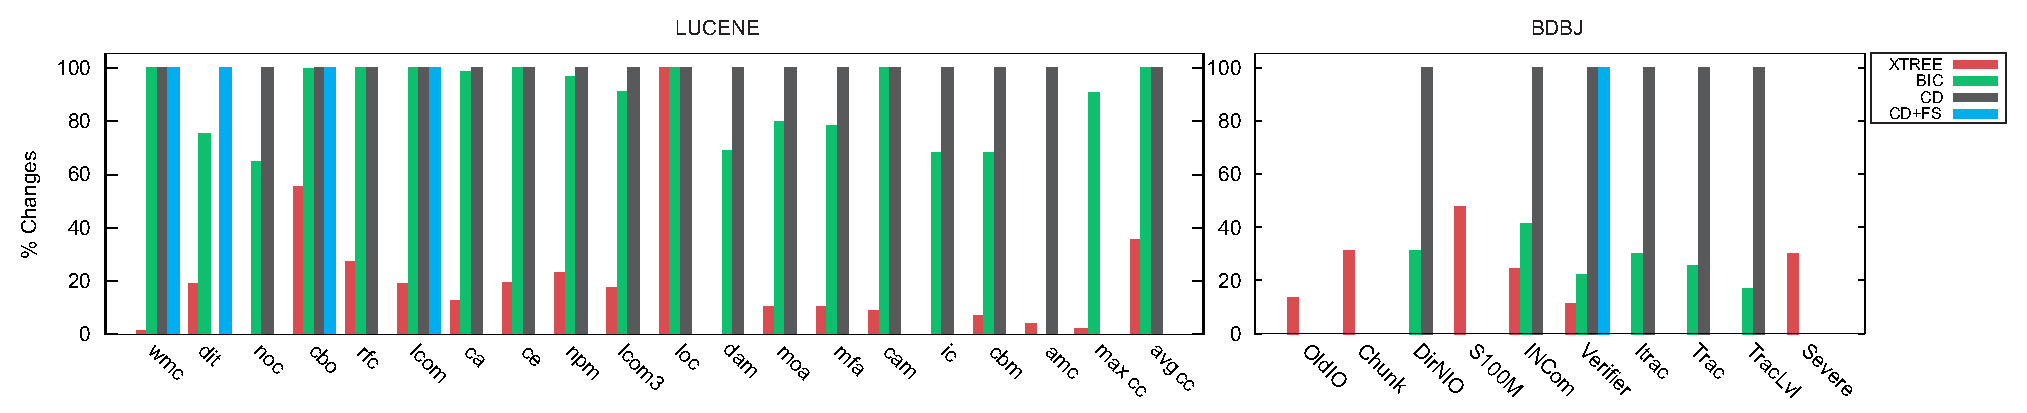
\includegraphics[width=\linewidth]{figs/Deltas-both.eps}
\caption{Percent frequency for how often certain feature was changed by a plan.}\label{fig:changed}
\end{figure*}

\subsubsection{Effectiveness Results}

 

Measured in terms of effectiveness,
some data sets were harder to optimize that others.  SQL (in \fig{conf1}) defied all 
our methods for reducing runtimes. Also, BDBJ (in \fig{conf1}) was hard to optimize
for all methods except XTREE.  However, in other data sets,
large reductions were observed:
\bi
\item
Down to 22\% of the original baseline in Ant of \fig{jur};
\item
Down to 6\% of the original baseline in BDBD  of \fig{conf1};
\ei
Overall, XTREE was most effective. It was always  the top-ranked method and (with 
the exception of SQL), had significant reductions in the median performance
values: median improvement of least 10\% lower (i.e. better) than the next ranked method.



\subsubsection{Succinctness Results}



\fig{changed} reports the percent of times in the 40 repeats that a method proposed changing a feature.
The left-hand-side plot of that figure reports results from one of the  Jureczko data sets ({\em lucene}) and the right-hand-side
  shows a Siegmund data set ({\em BDBJ}). 
  
  In these plots, the {\em more} succinct a planning method, the {\em less} percent
  of the runs
  where 
  it   recommends changing a particular feature (i.e. the vertical bars in that plot
  are {\em lower}). For example,
 Method1 (CD) was the least succinct  since it  wanted to change all features 
 (observe the change frequencies as 
high as 100\% for all features). 
Method1's policy of ``change everything''  might be acceptable
if this approach lead 
to the most effective changes. However, looking at 
\fig{jur} and  \fig{conf1}, there is no evidence for this.  

An  interesting feature of \fig{changed} was that fewer things 
were changed in the config data sets {\em BDBJ} than in the defect data set
{\em lucene}. 
In turns out that this holds true across nearly all our data sets.
\fig{types} summarizes all the change frequencies for all data sets. As with  \fig{changed},
there are fewer changed features in the config data than in the defect prediction data. 
One explanation for that is the nature of the features: the
defect data sets has continuous
features while the 
config data has binary independent features  (where so setting was turned ``on'' or ``off''). When exploring these different data types, it is possible to find more
\bi
\item
``Gentle slopes'' the lead to small changes
in  continuous space;
\item
 ``Sharp cliffs'' that lead to major change in the discrete
space. 
\ei
Hence, our planners can make fewer larger changes in the config data.
 For example, Method3 (BIC) and Method1 (CD) make far fewer changes in   data sets with discrete features (the Siegmund data) than in data with continuous features (the Jureczko data).  
 
 As to the method that lead to best effectiveness in \fig{jur} and \fig{conf1}, we note from \fig{types}
 that XTREE
 has a consistent behavior in both the discrete and continuous data sets.  Specifically,  in all our data sets,
 XTREE changes 
 usually changes around a fifth of the features.




\begin{figure}[!t]
\centering
{\small
\begin{tabular}{lcccc}
  \hline
  \rowcolor{lightgray}
       & DTREE & HOW   & kNN   & kNN+FS \\\hline
Ant    & 20.24\% & 86.84\% & 80.00\% & 10.00\%  \\
Ivy    & 20.88\% & 81.25\% & 70.00\% & 20.00\%  \\
Jedit  & 19.55\% & 92.27\% & 90.00\% & 20.00\%  \\
Lucene & 18.92\% & 85.64\% & 95.00\% & 25.00\%  \\
Poi    & 12.90\% & 79.45\% & 85.00\% & 20.00\%   \\\hline
\end{tabular}}
\noindent
\caption{Average change in attribute values}\label{fig:types}
\end{figure}



\subsubsection{Surprising Results}\label{sect:surprise}

If a planner only ever reports conclusions that were already known, then that planner offers
little value-added over ``just use established wisdom''. Accordingly, we studied our results
for plans that were somewhat counter-intuitive. 

Such a surprising plan can be  seen in the {\em lucene} results. Recall the standard advice for
OO systems: build classes that are internally cohesive with low coupling to other parts of the system~\cite{Dhama199565}. We can assess the relevance of this advice
to specific projects by checking how often a planner changes the
 coupling-related features:
\bi
\item {\em ca}:   afferent couplings  =  how many other classes use the specific
				class;
\item {\em  	ce}:  efferent couplings =  how many other classes is used by the
				specific class. 
\item {\em cbm}: coupling between methods =  total number of new/redefined methods
				to which all the inherited methods are coupled
\item	{\em cbo}:  coupling between objects = a value that increases when the methods of one
				class access services of another.
 
\item {\em ic}:   inheritance coupling =  number of parent classes to which a given
				class is coupled (includes counts of methods and variables inherited)
\ei
For the  {\em lucene} XTREE results  of  \fig{changed},
the most frequent change was to alter the lines of code in a class (see the tallest
red historgram in that figure on the {\em loc}, or lines of code). 
Looking at the logs of our planner, we can see
that XTREE's proposed changed is to {\em reduce} the size of a class.
The only way to do that,  while keeping the  same functionality, it is create a network
of smaller classes that interact to produce that functionality.
That is, we would need to {\em increase} the coupling of those classes to achieve XTREE's plan.

In theory, increasing coupling between classes complicates and confuses a class design.
But the {\em lucene} XTREE results  of  \fig{changed} rarely proposes changing   the
coupling features {\em ca, ce, cbm, ic} (in fact, XTREE never proposes any change to {\em ic}).

The only coupling issue that XTREE   usually adds to its plans is {\em cbo} (which appears 55\% of the time
in \fig{changed}). But note  that this is {\em object} coupling measure, not class coupling. So here
XTREE is warning against, say, some factory class generating a large
community of agents, all of the same class, who
co-ordinate on some task. This is a different issue to the class redesign issue that would
be triggered by altering {\em loc}.

In summary, XTREE satisfies that criteria that, sometimes, it produces surprising plans.
At least for the {\em lucense} data set, we can see advice that recommends {\em increasing coupling}
to reduce defects.

 


 
\section{Threats to Validity}\label{sect:valid}


As with any empirical study, biases can affect the final results. Therefore, any
conclusions made from this work must be considered with the following issues in
mind.


\subsection{ Learner Bias}
For building the defect predictors in this study, we elected
to use  Random Forest  and Random Forest Regressors .
We chose this approach,  based on its reputation for having the better  performance of 
21 other learners for defect prediction~\cite{lessmann}.
Data mining is a
large and active field and any single study can only use a small
subset of the known classification algorithms.  

That said, we have taken care to document in this paper the decisions made by engineering
judgement that could effect our conclusions. The above code used a set of variables which future
work should vary in order to test the internal validity of our conclusions:
\bi
\item All our planners divide data into groups of size $\alpha=\sqrt{N}$
\item Method2 used the top $\beta=33\%$ most informative features (ranked using INFOGAIN);
\item Method4 (XTREE) assumed that another sibling was useful if  had 
 a  score less than $\gamma=0.5$ times the mean score of the current leaf.
 \ei

\subsection{  Sampling bias} 
Sampling bias threatens any data mining experiment; i.e., what matters
there may not be true here. For example, the data sets used here comes from two sources
(Seigmund et al. and Jureczko et al.) and any biases in their selection procedures
threaten the validity of these results. 
That said,
the best we can do is define our methods and publicize our data and code so that other researchers can
try to repeat our results and, perhaps, point out a previously unknown bias
in our analysis. Hopefully, other researchers will emulate our methods in
order to repeat, refute, or improve our results. 



\subsection{  Evaluation Bias}\label{sect:coc}
Another threat to validity of this work is our use
of predictors learned on the training data to assess the impact of our planners.
This issues was discussed in detail in \tion{trust}. 

To those notes, we add a few more details. If possible, planners should be assessed via some external oracle that can accurately assess new examples. For example, in search-based software engineering,
examples can be assigned objective scores via  some model. In this approach, a changed example can be assessed by
generating actual objective scores from the model. 

\begin{figure}[!t]
%\noindent\begin{minipage}{0.5\textwidth} 
{\small 
\begin{tabular}{llrrc}
\arrayrulecolor{lightgray}
\rowcolor{lightgray}\textbf{Rank} & \textbf{Treatment} & \textbf{Median} & \textbf{IQR} & \\\hline
  1 &        XTREE &   59   &  9 & \quart{75}{4}{78}{99} \\
\hline   2 &      BIC &    5  & 1  & \quart{44}{0}{44}{99} \\
2 &          CD+FS & -7  & 100  & \quart{0}{53}{43}{99} \\   
2 &      CD &    -9  &  77 & \quart{21}{41}{42}{99} \\
\hline \end{tabular}}
\caption{Methods 1,2,3,4 applied to some ground-truth data (in this case, the POM3 model).
Values collected from  40 repeated runs of each method with different random seeds.
Results show the efficacy of XTREE in reducing the total overall cost in the original test data, when other planners fail to do so.}\label{fig:coc}
\end{figure}

For example, the COCOMO model from University of 
Southern California estimates software development time using a combination of industrial data and some domain expertise
from its author (Barry Boehm). \fig{coc} shows results from using COCOMO 
as an oracle to assess our planning methods. In this experiment, random projects were used as COCOMO
inputs. This generated an development time estimate for each example, which we passed to our four methods.
40 times, we let those methods propose changes to those projects. 
For assessment purposes, the changes projects were then feed back to the COCOMO
oracle. 

Using this approach, it is possible to assess the value of a plan by measuring its
effectiveness with respect to some ground truth (in this case, the COCOMO model).
As shown in \fig{coc}, XTREE passes this assessment.
Those results from the COCOMO model endorsed the conclusions of the rest
of this paper; i.e. compared to three other methods,  XTREE's supervised methods are best for generating plans on how to change
example projects.

\subsection{  Feasibility}\label{sect:feasibility}
It is important to also explore the general practicality of the plans. To this end, we are currently undertaking is a \textit{feasibility study} collaboration with industrial partners to assess the general feasibility of our changes. With this study, we would like to understand the nature of changes suggested by XTREE. Specifically: are the changes proposed by XTREE small enough to be easily implemented on software projects? Also, are the changes large enough to be feasible? In other words, we are asking if users can sufficient fine-grained control to make the changes proposed in \fig{changed}.
 
\section{Related work}

\subsection{Planning in AI}

The XTREE planner is somewhat different to the logical-based planners explored by 
classical AI. 
That kind of planning is a logical procedure~\cite{Fikes1971}
that seeks an ordering on {\em operators} to take some domain
{\em state} from a {\em start} state to a {\em  goal} state.
This classical logical approach is known to suffer from
computational bottlenecks~\cite{Bylander1994} while tools like XTREE will scale to any domains
that can generate decision trees.
  
\subsection{Evaluating Changes}

Some organizations have the resources to 
run repeated trials to assess  different treatments.
For example, in one remarkable recent study, Bente et al. report results
were the same for specification that was developed  by four different organizations~\cite{Anda2009}. Given those kind of resources, it would be possible
to (say) take a code base, assign it to different teams, make these teams  adopt different polices,
then check in 12 months time
 which teams have fewer defects than the others.  
 

Very few industrial or research groups have access
to the kinds of resources needed for this kind study  (evidence: in the six years since the
publication of that work, we know of only one   similar study to Bente et al.). Also, given the
diversity of modern software projects, it might be unreasonable to demand that all
proposed changes for all projects are always evaluated by something like the Bente et al. study.
Hence, 
this paper has used data miners to build an oracle that can assess changed examples. The advantage
of this approach is that it required far less resources to assess the effectiveness of proposed
changes to a project.  

\subsection{Search-based SE}

Another way way to propose changes to software artifacts
is   via some search-based method~\cite{Harman2009,Harman2011}. Such SBSE methods are   evolutionary programs that 
make
 extensive changes to  some initial sample of project data
 (perhaps 
100s to 100,000s of mutations). Each of these mutations
is reassessed using some domain model.
Examples of these algorithms include GALE, NSGA-II, NSGA-III, SPEA2, IBEA, particle swarm optimization, MOEA/D, etc.~\cite{krall14,deb00a,zit02,zit04,%
deb14,Cui2005a,zhang07:TEC}.

One problem with these   SBSE methods is that they can  make extensive mutations to the data they are exploring. In the language
of \tion{trust}, these methods may not be {\em trust-increasing} since those algorithms make no attempt
to mutate new examples away from the kinds of data used to commission the model (in which case, we would
start doubting the model's output).

Another issue with standard search-based SE methods is that they require ready access to 
trustworthy domain model that can offer an assessment
of newly generated examples. While some domains have such models (e.g. see the COCOMO effort estimation model
used in the last section), our experience is that many others do not.  For example, 
consider software defect prediction and all the intricate issues that may lead to defects in a product. A model that includes {\em all} those
potential issues would be very large and complex. Further,
the empirical data required to validate any/all parts
of that model can be hard to find.

What we would recommend is a two-pronged policy.
In domains with ready access to trusted models, we recommend
the kinds of tools that are widely used in the search-based
software engineering community such as GALE, NSGA-II, NSGA-III, SPEA2, IBEA, particle swarm optimization, MOEA/D, etc.~\cite{krall14,deb00a,zit02,zit04,%
deb14,Cui2005a,zhang07:TEC}. Otherwise, we recommend tools like XTREE.



\section{Summary}

The planner proposed in this paper propose changes to software project details in order to improve the expected
value of the performance scores of that part of the project.
To evaluate these planners,
data miners can be used to build oracles to assess planners.
Such planners should be {\em trust-increasing}; i.e. they propose changes that generate
changed examples that are closer to the training data of the data miner.
One caveat here is that the evaluations we can make on the planner are only as good as the predictive
performance of the data miner. Hence, if domain data does not support satisfactory predictors, then
planning in that domain cannot be evaluated.

Four planners were assessed here for the tasks of reducing defects and runtimes. 
Three of the methods come from our prior publications~\cite{me12c,krishna15}, and the conclusion of this
paper is that a novel fourth method clearly out-performs the other three
(measured in terms of {\em effectiveness, succinctness, and surprise}).
We conjecture that XTREE worked better than the rest since:
\bi
\item
It uses a supervised method to divide the data and;
\item
When planning how to move examples to better classes, it is   best to use a learner that reflects over 
differences between the classes.
\ei


\section{Questions for Future Work}

XTREE, as used here, sought improvements in a one goal (the   class variable). Does XTREE work for multi-goal reasoning?

 The XTREE algorithm seems quite general to any data of table with rows containing
weighted classes (so we can distinguish ``bad'' rows from ``better'' ones). 
Does   XTREE works  on   domains (other than the  defect/runtime data explored here)?

As an example of a domain that might benefit from XTREE, recent results raise doubts about
the value of changing code to remove ``bad smells''~\cite{Sjoberg13}. Can XTREE be used as a ``really bad smell''
detector to select the subset of possible refactorings that have the most   potential benefit?

As to scalability, XTREE is a post-processor to a decision tree algorithm. Hence, in theory,  XTREE should work on
any domain where data miners can generate decision trees. Given the current state of the art in Big Data,
can   XTREE  be applied to  very large data sets?

There are many more methods for generating plans and
no   one paper can survey them all. For example, this paper has not explored variations to the $\alpha,\beta,\gamma$
parameters that controlled XTREE. Would we get better results if we varied those parameters?

That said, the goal of this paper was not to claim that (e.g.) XTREE is some absolute optimal algorithm. Rather, it is
was to offer a baseline result (with XTREE) and an  evaluation strategy that  can assess  if alternate methods are better than XTREE.
Will other  researchers apply this strategy  to repeat and/or improve
(or even refute) our results?  Perhaps.

\section*{Acknowledgements}
The work has partially funded by a National Science Foundation CISE CCF award \#1506586.
\bibliographystyle{plain}


\balance
\bibliography{References}
\end{document}


  
  Next, build one centroid for each cluster (using the median and mode value for continuous
and discrete values, respectively).
After that, write a spreadsheet with one column per centroid;
\bi
\item
Sort the columns such that any current projects client fall into the left-most
columns. That is, make the left-hand-side of the sheet  ``current usual practice''
and the right-hand side  ``alternatives to current usual practice''.
\item
Sort the rows of that spreadsheet such that the rows with
maximum  variability appear at the top 
\ei
Now show the sheet to the business user, encouraging them to make recommendations by
\bi
\item
Comparing the left and right-sided columns;
\item
Using the features mentioned in the top-most rows (where changes selects for the most different centroids).
\ei

		
	
		

In theory, One  advantage of this method is that it focuses the attention of the business users
away from rows that do not select for different centroids and towards differences between
current usual practice and everything else.  
In the summer of 2011 and 2012, one of us (Menzies) spent two months
	working on-site at Microsoft Redmond,
	observing data mining analysts.  In that study, he took special
	note about how Microsoft's data scientists
	discussed the results of their data mining sessions with  business users. 
	
	One surprising observation was how  
	little time was spent by business users 
	inspecting  of the output of standard data miners. Prior to that visit,
	we had the mistaken impression that   decision trees,
	clustering algorithms, etc were useful ``off-the-shelf''; i.e    business
	users would inspect and understand the output of those tools.
	
Standard data mining tools are not necessarily the best tool for supporting that dialogue.
Menzies found that he had to do considerable work pre-processing data mining output
prior to the weekly briefing meetings for the business users. Initially,
that pre-processing was just clustering. This evolved into feature selection and finally
the a case-based reasoning tool called HOW.  


	
	as compared to another process, which we call {\em peeking}.
	In {\em peeking}, analysts and users spend much time
	inspecting and discussing small samples of either raw or exemplary or synthesized project data.  Further, very little of those discussions were  focused on classification
	(the addition of a labels to some unlabelled data). Rather, much time
	was spent in those meetings discussing {\em what to do next}; i.e. trying
	to determine what could be altered to better improve some business outcome.
	
	That   Microsoft  study found two common ``peeking'' methods.
	In {\em data engagement meetings},
	users debated the implications of data
	displayed on a screen. In this way, users
	engaged with the data and with each other by
	monitoring each others' queries and check each others'
	conclusions.
	
	Another data analysis pattern observed
	at Microsoft was  {\em cluster + contrast} in which
	data is  reduced to a few
	clusters. Users are then just shown the delta between those
	clusters. While contrasting, if feature values are
	the same in both clusters, then these were pruned from
	the reports to the user. In this way, very large
	data sets can be shown on one PowerPoint
	slide. Note that {\em cluster+contrast} is a tool that can be usefully employed within
	{\em data engagement meetings}.
	
	
	Cluster+contrast and engagement
	meetings are common practices at Microsoft. Yet  these methods had never been rigorously studied or certified.
	For both those reasons,
	we reflected over those tools to discover and analyze their
	underlying process. The result was HOW~\cite{howase}: a tool
	that combines (a)~feature selection; (b)~centroid generation from   clusters;
	(c)~contrast methods between centroids.
	While method (a) is widely used (e.g.~\cite{Menzies2010}),
	to the best of our knowledge, this combination of (abc) has not been thoroughly explored before.

This paper assesses two methods  for ``peeking'': a model-based method called DTREE and an instance-based method   called HOW. 
DTREE were first developed by Lekkalapudi and Menzies to  explaining results from multi-objective optimizers~\cite{nva14}. This paper is the first
to apply DTREE to defect prediction and contrast set learning. Also, that prior work evaluated
DTREE against multi-objective optimizers and not   instance-based methods.

This paper uses three criteria to assess the value of HOW and DTREE for
learning actionable analytics:
\be
\item
A planning system needs to be {\em effective}; i.e. if its recommendations
are applied then some statistically significant change should be observed.
To predict the number of defects in a data set before and after applying our changes,
we build a    prediction system (built by data mining; specifically: Random Forest). Note that this
predictor was built from some hold-out data (i.e. from  different data than that used
to build the predictor).
\item
Any  conclusion made to a business user must be understandable;
it must generate {\em succinct} changes.  
\item
Recommendations should be {\em stable}; i.e. they shouldn't widely vary due to minor changes in the data. Hence, in our experiments, we will add a little randomness to our analysis then report results across 20 repeated runs. 
\ee
We will find that
 {\em effectiveness} of DTREE and HOW are similar, but   DTREE wins on {\em succinctness} and {\em stability}.

\section{Cluster and Contrast}
\label{clust_contrast}
A recurring data analysis pattern in this paper is $cluster+contrast$. The data is distilled into a few clusters using a clustering scheme. Then lessons are inferred by studying the differences between these clusters. These lessons are used to generate rules that can be applied in any context.

\subsection{Clustering}
There are a wide variety of clustering methods to choose from. A study by Ganesan~\cite{div14} explored different clustering methods for software engineering data using the effort and defect data from the PROMISE repository~\cite{promise}. In that study methods such as WHERE, K-Means, mini-batch-K-Means, DBScan, EM, and Ward were investigated. The results of the study showed that the size and number of clusters is more important that the specifics of the techniques used. 

For this purposes of this work, we have chosen WHERE, a clustering scheme which is capable of generating at least $\sqrt{N}$ clusters given $N$ instances. In addition to this, WHERE has been shown to run fast while ignoring spurious dimensions~\cite{menzies2013}. This is particularly useful, for much of the SE data is noisy, they contain a information not associated with the target variable. 

\subsection{Finding Contrasts}
All the following methods use clustering in the form of WHERE, a top-down clustering method which recursively splits the data in two along a dimension that represents the highest variability. It works as follows:
\bi
\item Find   two   distance samples from the data, say  $X,Y$. This can be done by  picking any case $W$ at random, then setting $X$ to its most distant case, then setting $Y$ to the case most distant from $X$ (this requires only $O(2N)$ comparisons of $N$ cases).
\item Project each case $Z$ onto a {\tt Slope} that  runs between $X,Y$ using the cosine rule. 
\item Split the data at the median $X$ value of all cases and recurse on each half  (stopping when one half has less  than $\sqrt{N}$ of the original population).
\ei		

Clustering is followed by generating \textit{contrast sets}. These contrast sets represent recommendations on what could be altered to better improve an outcome. In this work we have explored several algorithms as possible tools to identify contrast between clusters. These fall into two broad categories:
\begin{enumerate}
\item Case Based Reasoning techniques (Nearest Neighbors and a gradient base planner called HOW)
\item Decision Trees.
\end{enumerate}

These techniques are discussed below. It is worth noting that the following techniques are organized in such a way that each one seeks to address certain shortcomings in the ones that precede it. 

\subsection{Case Based Reasoning}

Case-based reasoning seeks to find solutions to problems by emulating human recollection and adaptation from past experiences. It has found extensive usage in Artificial Intelligence because it offers several advantages. However, one of the most important benefits that CBR has to offer is that it works on a ``case-by-case'' basis. Therefore it's advise is tailored to be specific to the particular case being considered. Several paper in SE have applied this technique, most of all for effort estimation ~\cite{keung2008analogy, 6600685, walkerden1999empirical, shepperd1997estimating, kocaguneli2010use}. 

A classic example of a CBR is K Nearest Neighbor. Our version of nearest neighbor for planning is rather straight forward. It has been developed as a "straw-man"; i.e., a simple baseline tool to act as a benchmark used to evaluate other methods. 


\subsection{HOW}

HOW is very different compared to conventional CBR planners in that it explores the gradient between pairs of nearby clusters instead of studying the clusters themselves. HOW works by clustering the data during training using WHERE and then drawing \texttt{slopes} between the centroids of pairs of nearby clusters. Assuming the cluster pairs are labeled X and Y, with X having slightly better performance score than Y, the \texttt{slope} between X and Y acts as an indicator pointing to a direction in which to displace the data; i.e. away from Y and towards X. 

While testing, HOW finds the nearest slope to every test case. The slope provides the exact magnitude and direction of displacements. Contrast sets are derived from these displacements. HOW offers a distinct advantage over the other CBR planners by limiting the displacements to very small regions (the displacements are never more than the separation between two clusters). 

Although HOW manages to generate plans by localizing displacements to regions small enough to produce a statistically significant improvement, it needs to be noted that it fails to provide succinct summaries. Lack of succinctness makes it difficult draw generalizable conclusions about the test data. This is a trend commonly observed in most CBR systems. They tend to reason directly from a loaded training data instead of first summarizing the data into a model. 

% However, not all domains come with reliable models. For instance, a model that encompasses all the intricate issues that may lead to defects in software would be very large and indeed rather complex. In addition to this, finding empirical data to validate such models can be hard to come by and also time consuming ~\cite{me09i,me09j}. 

\subsection{DECISION TREES}

Trustworthy domain models are a popular alternatives to CBR planners. In our previous work, we have used executing source code as a "model" to check if our mutations to test suites minimize the test suite size while maximizing the number of statements covered~\cite{me09m,andrews07,andrews10}. However, we do not always have access to ready-to-use models. Further, finding empirical data to validate existing models can be hard. 

Taking into account the wealth of data that is available to us, this issue can fortunately be circumvented by constructing a categorical model based on decision trees. Unlike the previous planners which use where, here we construct a decision tree using information gain as a metric to find ideal splits in the data. This allows us to identify the most informative attributes to select. A decision tree (hereafter referred to as DTREE) built in this fashion emulates a model built from the training data. 

Using DTREE, the test cases can be categorized into one of the branches of the tree. Now, to generate the contrast sets, we determine (1) What \textit{current} branch does a test case fall in?; (2) What \textit{desired} branch would the test case have to move to?; (3) What are the deltas between \textit{current} and \textit{desired}? The last question can be answered by finding the deltas in branches of the decision tree that lead to \textit{desired} from \textit{current}. For full algorithmic details, refer to \fig{xtrees_bare}.

A tree structure such as DTREE is characterized by attributes such as size and depth. It is worth noting that these attributes have a profound impact on its performance. Our initial motivation for using DTREE was that they could serve as a medium for experts to reason about a data. The size of the tree, if too large, jeopardizes the readability of the solutions by increasing the complexity. We have, therefore, endeavored to reduce the size of the tree by pruning away irrelevant solutions that do not contribute to better solutions (refer to step-2 of \fig{xtrees_bare}). 

DTREE offers a great number of benefits compared to the other methods that were discussed above. Firstly, it offers a visual medium for experts to identify and explore solutions spaces that are local to the problem. Secondly, its solutions are much more stable than other cluster specific and instance specific learners. This stability can be attributed to the consistency and general reproducibility of the tree structure. Thirdly, and perhaps most importantly, the tree summarizes the training data succinctly, making it easier for a business user to examine the solution sets.

\lstnewenvironment{code}[1]{
\lstset{
mathescape,
numbers=left,
numberstyle=\scriptsize,
stepnumber=1,
numbersep=0.5em,
xleftmargin=1em,
framextopmargin=2em,
framexbottommargin=2em,
showspaces=false,
showtabs=false,
showstringspaces=false,
tabsize=2,
% Basic
basicstyle=\ttfamily\scriptsize,
backgroundcolor=\color{Background},
language=Python,
% Comments
commentstyle=\color{Comments}\slshape,
% Strings
stringstyle=\color{Strings},
morecomment=[s][\color{Strings}]{"""}{"""},
morecomment=[s][\color{Strings}]{'''}{'''},
% keywords
morekeywords={[1]import,from,class,def,for,while,if,is,in,elif,else,not,and,or,print,break,continue,return,True,False,None,access,as,,del,except,exec,finally,global,import,lambda,pass,print,raise,try,assert, dot, norm, zip, sorted},
keywordstyle={[1]\color{Code}\bfseries},
% additional keywords
morekeywords={[3]fastmap,Slope,bPruning,clister,train,leafs,weightedFeatures,HOW,envy, score,kNN,contrastSet,exemplar,Prune, FSel, exemplar,nearestSlope,dist,displace,geometry,splitAcross2Points,leaves,How,nearest,bPruning,Stats,divide,recurse,weight1,project, furthest, split,WHERE,clusterer, getContours,envied, fWeight, nearestContour, projection, mutate, HERE, knn},
keywordstyle={[3]\color{Keywords}\bfseries},
morekeywords={[2]@invari},
keywordstyle={[2]\color{Decorators}\slshape},
emph={self},
emphstyle={\color{self}\slshape},
firstnumber=last
%
}}{}
